% !TeX program = xelatex
\documentclass[12pt,a4paper,oneside]{report}
\usepackage{fontspec}
\IfFontExistsTF{Times New Roman}{\setmainfont{Times New Roman}}{\setmainfont{TeX Gyre Termes}}
\setmonofont{Latin Modern Mono}
\usepackage{graphicx,amsmath,amssymb,booktabs,tabularx,tikz,url}
\usepackage{xurl}
\usetikzlibrary{calc}
\usepackage[left=30mm,right=20mm,top=25mm,bottom=25mm,footskip=13mm]{geometry}
\usepackage{titlesec,tocloft}
\usepackage[font=small,labelfont=bf]{caption}
\usepackage[hidelinks,unicode]{hyperref}
\linespread{1.17}
\setlength{\emergencystretch}{2em}
\renewcommand{\arraystretch}{1.14}
\setlength{\parindent}{1.65em}
\setlength{\parskip}{.25em}
\renewcommand{\chaptername}{Chương}
\renewcommand{\appendixname}{Phụ lục}
\renewcommand{\contentsname}{Mục lục}
\renewcommand{\listfigurename}{Danh sách hình vẽ}
\renewcommand{\listtablename}{Danh sách bảng}
\renewcommand{\figurename}{Hình}
\renewcommand{\tablename}{Bảng}
\renewcommand{\bibname}{Tài liệu tham khảo}
\makeatletter
\newcommand{\ChapterCaption}{\@chapapp}
\makeatother
\titleformat{\chapter}[hang]{\normalfont\LARGE\bfseries}{\ChapterCaption\ \thechapter.}{.45em}{}
\titleformat{name=\chapter,numberless}[hang]{\normalfont\LARGE\bfseries}{}{0pt}{}
\titlespacing*{\chapter}{0pt}{0pt}{32pt}
\titlespacing*{\section}{0pt}{15pt}{5pt}
\titlespacing*{\subsection}{0pt}{10pt}{4pt}
\renewcommand{\cftchappresnum}{Chương\ }
\renewcommand{\cftchapaftersnum}{.}
\setlength{\cftchapnumwidth}{5.1em}
\renewcommand{\cftchapleader}{\cftdotfill{\cftsecdotsep}}
% Tên đề tài do sinh viên cung cấp.
\newcommand{\DonVi}{ĐẠI HỌC QUỐC GIA HÀ NỘI}
\newcommand{\Truong}{TRƯỜNG ĐẠI HỌC CÔNG NGHỆ}
\newcommand{\SinhVien}{Nguyễn Hữu Thái Dương}
\newcommand{\MaSinhVien}{23021789}
\newcommand{\TenDeTai}{Nghiên cứu đánh giá hiệu năng các bộ lọc ước lượng trạng thái phi tuyến trong bài toán theo dõi phương tiện giao thông trên nền tảng nhúng Jetson Nano}
\newcommand{\LoaiQuyen}{Đồ án tốt nghiệp đại học hệ chính quy}
\newcommand{\Nganh}{Công nghệ kỹ thuật điện tử - viễn thông}
\newcommand{\HuongDan}{Tiến sĩ Hoàng Gia Hưng}
\newcommand{\DongHuongDan}{} % Để trống nếu không có.
\newcommand{\NoiNam}{HÀ NỘI -- 2026}


% Hình thức bìa theo hai mẫu PDF người dùng cung cấp.
\newcommand{\trangbia}[1]{%
  \thispagestyle{empty}\null
  \begin{tikzpicture}[remember picture,overlay]
    \draw[line width=1.05pt] ($(current page.north west)+(24.5mm,-20mm)$)
      rectangle ($(current page.south east)+(-15mm,24.5mm)$);
    \draw[line width=.35pt] ($(current page.north west)+(26mm,-21.5mm)$)
      rectangle ($(current page.south east)+(-16.5mm,26mm)$);
    \coordinate (center) at ($(current page.north)+(4.75mm,0)$);
    \node[anchor=north,align=center,font=\bfseries] at ($(center)+(0,-25mm)$)
      {\DonVi\\[2mm]\Truong};
    \ifnum#1=0\relax
      \node at ($(center)+(0,-75mm)$){
\includegraphics[height=31mm]{hinh/logo-uet.png}};
    \fi
    \node[align=center,font=\large\bfseries] at ($(center)+(0,-102mm)$){\SinhVien};
    \node[align=center,text width=154mm,font=\Large\bfseries] at ($(center)+(0,-135mm)$)
      {\MakeUppercase{\TenDeTai}};
    \node[align=center,font=\large\bfseries] at ($(center)+(0,-176mm)$)
      {\MakeUppercase{\LoaiQuyen}\\[2mm]Ngành\enspace \Nganh};
    \ifnum#1=1\relax
      \node[anchor=north west,align=left,font=\large\bfseries] at ($(current page.north west)+(36mm,-200mm)$)
        {Cán bộ hướng dẫn\enspace \HuongDan
         \ifx\DongHuongDan\empty\else\\[6mm]Cán bộ đồng hướng dẫn\enspace \DongHuongDan\fi};
    \fi
    \node[font=\bfseries] at ($(center)+(0,-255mm)$){\NoiNam};
  \end{tikzpicture}\clearpage}

\hypersetup{pdftitle={\TenDeTai},pdfauthor={\SinhVien}}
\begin{document}
\hypersetup{pageanchor=false}
\pagestyle{empty}
\trangbia{0}
\trangbia{1}
\newcommand{\tieudephandau}[1]{\begin{center}\Large\bfseries #1\end{center}\vspace{.75em}}
\tieudephandau{TÓM TẮT}
Theo dõi phương tiện qua video cần duy trì mã định danh khi xe đổi hướng, xuất hiện trở lại sau che khuất hoặc chỉ chiếm một vùng nhỏ trên ảnh. Khóa luận xây dựng hệ thống theo dõi dựa trên phát hiện, kết hợp YOLO với ByteTrack. Nghiên cứu so sánh bộ lọc Kalman tuyến tính với mô hình vận tốc không đổi cùng ba cấu hình EKF, UKF và PF sử dụng mô hình tốc độ và tốc độ quay không đổi. Mỗi phép so bộ lọc dùng chung đầu ra detector và quy tắc ghép. Chất lượng phát hiện, theo dõi và tốc độ được đo theo các giao thức riêng.

Trên RoundaboutHD, EKF và UKF cùng giảm số lần đổi ID từ 34 xuống 28 trong nhóm xe đổi hướng từ $25^\circ$. Ở nhóm khả kiến thấp của 40 đoạn UA-DETRAC, KF, EKF và UKF lần lượt có 53, 50 và 48 lần đổi ID, với số bỏ sót gần như bằng nhau. KF có số lần đổi ID thấp nhất khi tính toàn cửa sổ trên hai phép so này. Trên toàn bộ 182 clip test HELMET, số lần đổi ID tương ứng là 717, 444 và 452. Hiệu quả của mô hình chuyển động phụ thuộc vào kịch bản và chất lượng phát hiện.

Trên Jetson Nano, cấu hình YOLO11n 50/50 FP16, lọc trước NMS, NMS ma trận và giải mã JPEG gối đầu nâng tốc độ trung bình từ 13,12 lên 18,63 FPS trên 80 đoạn BDD100K và UA-DETRAC với KF. Cả 80 đoạn đạt mốc 15 FPS khi suy luận đủ khung, dùng chuỗi JPEG và tắt hiển thị. Trung vị độ trễ p90 theo đoạn tăng từ 90,08 lên 123,88 ms. Trong phép đối chiếu bốn bộ lọc trên 16 đoạn, KF và EKF đạt mốc 15 FPS ở cả 16 đoạn, UKF đạt 14 đoạn và RBPF500 đạt sáu đoạn.
\par\medskip\noindent\textbf{Từ khóa:} theo dõi đa đối tượng, ByteTrack, Kalman, bộ lọc hạt, phương tiện giao thông, Jetson Nano.

\clearpage\tieudephandau{LỜI CAM ĐOAN}
Tôi cam đoan các số liệu và kết quả trong đồ án được trình bày theo hồ sơ thực nghiệm được dẫn chiếu. Các phương pháp, bộ dữ liệu và công trình có sử dụng đều được ghi nguồn tại nội dung liên quan và danh mục tài liệu tham khảo. Tôi chịu trách nhiệm về nội dung của bản đồ án đã kiểm tra và nộp.
\begin{flushright}
Hà Nội, ngày \rule{9mm}{.35pt} tháng \rule{9mm}{.35pt} năm 2026\\[5pt]
Tác giả\\[28mm]
\textbf{\SinhVien}\\
Mã sinh viên\enspace \MaSinhVien
\end{flushright}

\clearpage\tieudephandau{LỜI CẢM ƠN}
Em xin chân thành cảm ơn các thầy, cô của Trường Đại học Công nghệ, Đại học Quốc gia Hà Nội đã trang bị cho em kiến thức và phương pháp học tập trong suốt thời gian đào tạo.

Em xin cảm ơn cán bộ hướng dẫn đã góp ý về cách thiết kế phép so sánh, cách kiểm chứng kết quả và phạm vi triển khai hệ thống. Những góp ý này giúp em làm rõ mối quan hệ giữa chất lượng phát hiện, độ ổn định định danh và chi phí xử lý trên thiết bị nhúng.

Em cũng xin cảm ơn những người đã hỗ trợ em trong quá trình học tập và hoàn thành đồ án.
\begin{flushright}\textbf{\SinhVien}\end{flushright}

\clearpage\pagenumbering{roman}\pagestyle{plain}\tableofcontents
\clearpage\listoffigures
\clearpage\listoftables
\clearpage\tieudephandau{DANH MỤC TỪ VIẾT TẮT}
\noindent\begin{tabularx}{\textwidth}{@{}lX@{}}
\toprule\textbf{Từ viết tắt} & \textbf{Diễn giải}\\\midrule
AP & Average Precision, độ chính xác trung bình\\
COCO & Common Objects in Context, tập dữ liệu vật thể trong ngữ cảnh\\
CTRV & Constant Turn Rate and Velocity, mô hình tốc độ và tốc độ quay không đổi\\
CV & Constant Velocity, mô hình vận tốc không đổi\\
EKF & Extended Kalman Filter, bộ lọc Kalman mở rộng\\
ESS & Effective Sample Size, số hạt hiệu dụng\\
FN & False Negative, lượt đối tượng bị bỏ sót\\
FP & False Positive, lượt dự đoán không khớp nhãn\\
FPS & Frames Per Second, số khung xử lý mỗi giây\\
GT & Ground Truth, nhãn chuẩn dùng để đánh giá\\
HOTA & Higher Order Tracking Accuracy, chỉ số chất lượng theo dõi\\
IDF1 & Điểm F1 theo danh tính\\
IDSW & Identity Switches, số lần đổi mã định danh\\
IoU & Intersection over Union, tỷ lệ diện tích giao trên diện tích hợp\\
KF & Kalman Filter, bộ lọc Kalman\\
mAP & Mean Average Precision, trung bình AP theo lớp\\
MOT & Multiple Object Tracking, theo dõi đa đối tượng\\
NMS & Non-Maximum Suppression, loại bỏ hộp dự đoán chồng lấp\\
PF & Particle Filter, bộ lọc hạt\\
UKF & Unscented Kalman Filter, bộ lọc Kalman dùng biến đổi unscented\\
YOLO & You Only Look Once, họ bộ phát hiện đối tượng\\\bottomrule
\end{tabularx}

\clearpage\pagenumbering{arabic}\pagestyle{plain}\hypersetup{pageanchor=true}
\chapter{Mở đầu}
\section{Một lần mất dấu ở giao lộ}
Xét hai xe máy đi sát nhau trước đầu xe buýt. Ở khung hình đầu, cả hai xe máy đều có hộp phát hiện. Vài khung hình sau, xe buýt che một xe máy đang rẽ. Khi xe này xuất hiện trở lại, bộ phát hiện có thể vẽ đúng hộp bao quanh nó mà hệ thống vẫn gán sai mã định danh. Với bài toán đếm phương tiện, một hành trình có thể bị đếm hai lần. Với bài toán khôi phục quỹ đạo, đoạn trước và sau xe buýt sẽ thuộc hai bản ghi khác nhau. Đây là tình huống minh họa cho sự khác nhau giữa phát hiện một xe và theo dõi cùng một xe qua thời gian.

Trong khoảng bị che, hệ thống có hai nguồn thông tin. Trạng thái tích lũy trước đó cho biết xe có khả năng đi đâu. Hộp phát hiện mới, nếu có, cho biết phương tiện có thể đang ở vị trí nào. ByteTrack nối hai nguồn thông tin bằng phép ghép quỹ đạo với phát hiện \cite{zhang2022bytetrack}. Bộ lọc chuyển động tham gia trực tiếp vào phép ghép qua vị trí và kích thước hộp dự đoán. Tuy nhiên một dự đoán tốt cũng có thể mất ID nếu xe khác chiếm phép ghép hoặc nếu quỹ đạo đã hết thời gian chờ.

\section{Từ SORT đến câu hỏi về bộ lọc}
SORT kết hợp bộ lọc Kalman với bài toán gán giữa các khung hình. Bewley và cộng sự chỉ ra rằng việc đổi bộ phát hiện có thể làm thay đổi đáng kể kết quả theo dõi \cite{sort}. ByteTrack mở rộng cách dùng các phát hiện bằng việc thử ghép những hộp có điểm thấp với các quỹ đạo còn đủ điều kiện. Một hộp xe bị che một phần có thể không đủ tin cậy để khởi tạo quỹ đạo nhưng vẫn giúp nối tiếp một quỹ đạo đã có. Hai nghiên cứu gợi ra hai phép đối chứng khác nhau cho khóa luận. Khi khảo sát mô hình chuyển động, cần cho các bộ lọc đọc cùng một danh sách phát hiện. Khi so sánh hai bộ theo dõi, cần giữ cùng bộ lọc và điều kiện đầu vào.

Mô hình vận tốc không đổi dự đoán tâm xe tiếp tục đi theo hướng vừa quan sát. Mô hình có tốc độ quay cho phép tâm xe đi theo một cung tròn. Khả năng biểu diễn này đặc biệt đáng khảo sát ở nút giao, nhưng bản thân độ cong của mô hình chưa bảo đảm một ID sẽ được giữ lâu hơn. Tâm hộp trên ảnh còn phụ thuộc phối cảnh, góc quay camera và phần thân xe nhìn thấy. Khi xe mới xuất hiện, chỉ một phép đo vị trí không đủ xác định đồng thời hướng đi và tốc độ quay.

\section{Câu hỏi và phương pháp}
Khóa luận đặt ra ba câu hỏi. Thứ nhất, khi đầu vào phát hiện đã cố định, thay KF/CV bằng EKF, UKF hoặc PF dùng mô hình CTRV làm thay đổi chất lượng theo dõi bao nhiêu? Thứ hai, các bộ lọc có giữ ID tốt hơn khi xe đổi hướng, có khả kiến thấp hoặc thuộc lớp xe máy không? Thứ ba, có thể đạt 15 FPS trên Jetson Nano trong điều kiện nào và chất lượng phát hiện, theo dõi và độ trễ thay đổi ra sao?

Để trả lời hai câu đầu, nghiên cứu lưu phát hiện theo video, phát lại chúng cho từng bộ lọc rồi chấm quỹ đạo theo cùng một bộ nhãn. Đánh giá chính sử dụng UA-DETRAC và BDD100K, hai bộ dữ liệu có điều kiện ghi hình và quy ước nhãn khác nhau \cite{detrac,bdd}. Phân tích theo tình huống dùng RoundaboutHD cho xe đổi hướng, UA-DETRAC cho che khuất và HELMET cho xe máy. SVMOT cung cấp phép đối chiếu khả kiến thấp ở miền khác. Phép thử UTUAV kiểm tra chuyển miền sang góc nhìn từ trên cao. Phép đo trên Jetson Nano dùng cùng 80 đoạn cho hai cấu hình detector và chấm đầu ra bằng nhãn gốc.

\section{Đóng góp và phạm vi}
Đóng góp thứ nhất là một đường thực nghiệm từ huấn luyện detector năm lớp đến chấm quỹ đạo. Đường này giữ được quan hệ giữa checkpoint, phát hiện theo khung hình và kết quả theo video. Đóng góp thứ hai là các phép so ghép cặp giữa bốn cấu hình chuyển động, có kiểm tra ảnh hưởng của seed đối với PF, kèm phân tích dự đoán và liên kết khi PF giảm điểm trên RoundaboutHD. Đóng góp thứ ba là phép đo trên Nano tách thời gian chạy mạng khỏi tốc độ toàn hệ thống, đi kèm đối chiếu chất lượng khi đổi hình dạng ảnh.

Nghiên cứu theo dõi ID trong từng camera và ước lượng chuyển động trên mặt phẳng ảnh. Kết luận riêng về xe máy rẽ phụ thuộc số quỹ đạo có nhãn cho tình huống đó.

\section{Bố cục khóa luận}
Chương 2 trình bày mô hình chuyển động và chỉ số đánh giá. Chương 3 mô tả dữ liệu huấn luyện, các thành phần của hệ thống và giao thức. Chương 4 trình bày độ chính xác detector, kết quả theo dõi và phân tích theo tình huống. Chương 5 trình bày tối ưu Jetson Nano và đánh đổi về chất lượng, tốc độ và độ trễ. Chương 6 tổng kết kết quả và hướng phát triển.

\chapter{Cơ sở lý thuyết}
\section{Quan sát và danh tính}
Tại khung hình $t$, detector trả về tập $D_t$ gồm vị trí, lớp và điểm tin cậy của từng hộp. Một hộp có tâm $(c_x,c_y)$, chiều rộng $w$ và chiều cao $h$. Phép đo dùng cho bộ lọc là $z=(c_x,c_y,a,h)^\top$, với $a=w/h$. Một quỹ đạo mang ID, trạng thái ước lượng và thời điểm cập nhật gần nhất. Hai ô tô có thể cùng lớp và có hộp gần như trùng nhau. Vì vậy, nhãn lớp riêng lẻ không xác định được danh tính.

Mỗi bước gồm dự đoán, liên kết và cập nhật. Phép đo chỉ được đưa vào bộ lọc sau khi quỹ đạo đã ghép được với một phát hiện. Một hộp dự đoán lệch khỏi xe thật có thể làm mất chính phép đo cần để hiệu chỉnh sai số. Sai số dự đoán và lỗi liên kết vì thế có quan hệ hai chiều qua các khung hình kế tiếp.

\section{Ghép quỹ đạo trong ByteTrack}
Độ chồng lấp giữa hai hộp $B_1,B_2$ được đo bằng $\mathrm{IoU}=|B_1\cap B_2|/|B_1\cup B_2|$. Với hai hộp bằng nhau chỉ dịch ngang một đoạn $d$ nhỏ hơn chiều rộng $w$, IoU bằng $(w-d)/(w+d)$. Cùng một độ lệch mười pixel, hộp rộng 30 pixel có IoU bằng 0,50, trong khi hộp rộng 100 pixel còn khoảng 0,82. Sai số tâm theo pixel do đó có ý nghĩa khác nhau đối với xe xa và xe gần.

ByteTrack dự đoán hộp của các quỹ đạo hiện có và ghép trước với nhóm phát hiện có điểm cao. Phép gán một-một xét các ứng viên đồng thời. Từng quỹ đạo không được tự chọn cùng một phát hiện. Ở lượt thứ hai, các quỹ đạo đang theo dõi còn đủ điều kiện có thể ghép với hộp có điểm thấp \cite{zhang2022bytetrack}. Bước này hữu ích khi bộ phát hiện còn nhìn thấy một phần xe. Khi detector bỏ sót hoàn toàn, quỹ đạo chỉ có thể chờ một phép đo về sau trong khoảng thời gian cho phép. Một quỹ đạo đã mất và một quỹ đạo đang hoạt động vì thế có thể có các cơ hội ghép khác nhau.

\section{Kalman với vận tốc không đổi}
Đặt $u=(c_x,c_y,a,h)^\top$. Cấu hình đối chứng dùng trạng thái $x=(u^\top,\dot u^\top)^\top$. Tại bước $\Delta t$, mô hình tuyến tính có dạng
\[
 x_{t|t-1}=F x_{t-1|t-1},\quad
 F=\begin{pmatrix}I&\Delta t I\\0&I\end{pmatrix},\qquad H=(I\quad 0).
\]
Các ma trận $Q$ và $R$ lần lượt mô tả nhiễu quá trình và nhiễu đo. Phương sai dự đoán $P^- = FPF^\top+Q$ tăng theo độ bất định của mô hình. Khi ghép được $z_t$, phép hiệu chỉnh Kalman \cite{kalman} dùng
\[
 S=HP^-H^\top+R,\qquad K=P^-H^\top S^{-1},\qquad
 x^+=x^-+K(z_t-Hx^-).
\]
Nếu bất định phép đo lớn so với bất định dự đoán, hệ số hiệu chỉnh theo hướng đó nhỏ. Trong thời gian thiếu quan sát, bước cập nhật không diễn ra. Ở đây $\Delta t$ được đo bằng bước khung hình. Cần tách đại lượng này khỏi thời gian vật lý, đặc biệt khi đối chiếu video 5 và 30 khung hình mỗi giây.

\section{Mô hình quay trên mặt phẳng ảnh}
Trạng thái CTRV của hệ thống có chín thành phần
\[
 x=(c_x,c_y,v,\theta,\omega,a,h,\dot a,\dot h)^\top .
\]
Tốc độ $v$ đo bằng pixel trên bước, hướng $\theta$ đo bằng radian và tốc độ quay $\omega$ đo bằng radian trên bước. Trong một bước, coi $v$ và $\omega$ không đổi, đặt $\theta'=\theta+\omega\Delta t$. Khi tốc độ quay khác không, tích phân hai thành phần vận tốc theo trục ảnh cho
\begin{align}
 c'_x &=c_x+\frac{v}{\omega}(\sin\theta'-\sin\theta),\\
 c'_y &=c_y+\frac{v}{\omega}(\cos\theta-\cos\theta').
\end{align}
Khi $|\omega|$ gần 0, phép tính dùng giới hạn đi thẳng với gia số $v\Delta t(\cos\theta,\sin\theta)$. Cách viết này tránh phép chia cho số rất nhỏ. Tỷ lệ $a$ và chiều cao $h$ tiếp tục tiến triển tuyến tính theo $\dot a,\dot h$. Bốn thành phần có thể quan sát trực tiếp vẫn là $c_x,c_y,a,h$.

Ví dụ, ở bước đầu hai quỹ đạo có cùng tâm và cùng vận tốc tiếp tuyến sẽ có dự đoán gần nhau. Sau nhiều bước không có phép đo, CV tiếp tục theo tiếp tuyến, còn CTRV tích lũy góc quay. Nếu tốc độ quay được ước lượng đúng, dự đoán CTRV còn gần xe đang rẽ. Nếu tốc độ quay chủ yếu phản ánh dao động hộp phát hiện, cùng cơ chế tích lũy góc có thể khiến hộp dự đoán trôi nhanh hơn. Đây là lý do phải kiểm tra sai số theo số khung hình thiếu quan sát.

\section{EKF và UKF trên cùng hàm chuyển}
EKF tính $x^-=f(x)$ và lấy Jacobian $J_f$ tại trạng thái hiện thời để truyền hiệp phương sai $P^-=J_fPJ_f^\top+Q$. Hướng và tốc độ quay tác động đến hai tọa độ tâm qua các hàm lượng giác. Khi độ bất định nhỏ, đạo hàm cục bộ cho cách tính gọn. Khi trạng thái phân tán trên nhiều hướng, một tiếp tuyến tại tâm có thể đại diện kém cho phân bố sau biến đổi.

UKF dùng biến đổi unscented \cite{julier}. Với trạng thái chín chiều, thuật toán tạo 19 điểm sigma từ trung bình và hiệp phương sai hiện tại. Mỗi điểm đi qua cùng hàm $f$, sau đó các trọng số khôi phục trung bình và hiệp phương sai dự đoán. Riêng với hướng, trung bình của hai góc $179^\circ$ và $-179^\circ$ phải ở gần $180^\circ$. Hệ thống tính trung bình vòng bằng tổng có trọng số của sin và cos, rồi đưa hiệu góc về cùng một chu kỳ khi tính phương sai. Vì phép đo chỉ chọn tọa độ, nó là phép biến đổi tuyến tính ngay cả khi bước dự đoán phi tuyến. So EKF với UKF vì thế trực tiếp khảo sát cách truyền bất định qua bước chuyển động.

\section{Bộ lọc hạt}
Bộ lọc hạt biểu diễn trạng thái bằng tập $\{(x_i,w_i)\}_{i=1}^{N}$ với $\sum_i w_i=1$. Trong bộ lọc bootstrap \cite{gordon}, mỗi hạt được truyền qua mô hình rồi cộng nhiễu quá trình. Khi có phép đo, hạt có hộp phù hợp được tăng trọng số tương đối. Với phép đo Gaussian, bước cập nhật trọng số có dạng
\[
 \log\widetilde w_i=\log w_i-\tfrac12(z-Hx_i)^\top R^{-1}(z-Hx_i)+C.
\]
Hằng số chung $C$ mất đi khi chuẩn hóa. Triển khai tính trong miền log để tránh làm tròn các xác suất nhỏ về 0. Phép ghép của ByteTrack vẫn cần một hộp duy nhất. Cấu hình PF500 lấy trung bình có trọng số, vì vậy việc duy trì nhiều hạt chưa đồng nghĩa với việc bộ ghép xét nhiều hộp cho cùng một xe.

Số hạt hiệu dụng $N_{\mathrm{eff}}=1/\sum_i w_i^2$ bằng $N$ khi các trọng số đều và tiến gần 1 khi một hạt chiếm gần hết trọng số. Hệ thống lấy mẫu lại có hệ thống khi $N_{\mathrm{eff}}<0{,}5N$. Các hạt mới trở về trọng số đều, nhưng nhiều hạt có thể cùng xuất phát từ một trạng thái. Do đó, số hạt hiệu dụng, độ trải theo vị trí và sai số tâm cần được xem cùng nhau. Chỉ quan sát tần suất lấy mẫu lại chưa cho biết nguyên nhân một quỹ đạo bị đứt.

\section{Đo chất lượng ở hai tầng}
Ở tầng phát hiện, precision là tỷ lệ phát hiện đúng trong các hộp dự đoán và recall là tỷ lệ đối tượng có nhãn được tìm thấy. AP tổng hợp đường precision--recall khi thay ngưỡng điểm. mAP50 lấy trung bình AP theo lớp ở IoU 0,50. mAP50--95 còn lấy trung bình qua các ngưỡng IoU từ 0,50 đến 0,95, cách nhau 0,05. Do đó một detector tìm thấy nhiều xe nhưng dự đoán mép hộp chưa sát có thể tăng mAP50 nhiều hơn mAP50--95.

Ở tầng quỹ đạo, HOTA kết hợp độ chính xác phát hiện và độ chính xác liên kết \cite{hota}. Tại một ngưỡng khớp $\alpha$,
\[
 \mathrm{DetA}_\alpha=\frac{\mathrm{TP}_\alpha}{\mathrm{TP}_\alpha+\mathrm{FP}_\alpha+\mathrm{FN}_\alpha},
 \qquad \mathrm{HOTA}_\alpha=\sqrt{\mathrm{DetA}_\alpha\,\mathrm{AssA}_\alpha}.
\]
AssA đánh giá một cặp danh tính khớp nhau nhất quán tới đâu trong suốt quỹ đạo. HOTA cuối lấy trung bình theo các ngưỡng. Điểm COMBINED được tổ hợp từ các thành phần do bộ chấm trả về, nên video dài có nhiều đối tượng không mặc nhiên có cùng trọng số với một video ngắn có ít xe.

IDF1 đo mức khớp danh tính qua $2\,\mathrm{IDTP}/(2\,\mathrm{IDTP}+\mathrm{IDFP}+\mathrm{IDFN})$ \cite{ristani}. IDSW đếm lần đổi ID theo quy tắc của bộ chấm. MOTA dùng $1-(\mathrm{FN}+\mathrm{FP}+\mathrm{IDSW})/\mathrm{GT}$ và có thể âm khi số lỗi lớn hơn số hộp chú thích qua các khung hình. IDSW thấp cũng có thể do hệ thống chỉ theo dõi được rất ít xe. Khóa luận vì vậy đọc số lần đổi ID cùng IDF1, số hộp bỏ sót và độ phủ của mẫu.

\chapter{Thiết kế và triển khai hệ thống}
\section{Tách phát hiện khỏi theo dõi}
\begin{figure}[htbp]\centering
\fbox{\begin{minipage}{0.87\linewidth}\centering
Video và nhãn theo từng camera\\[3pt]
$\downarrow$\\
Bộ phát hiện YOLO $\longrightarrow$ bộ nhớ đệm theo video\\[3pt]
$\downarrow$\\
Lọc theo lớp và điểm $\longrightarrow$ ByteTrack + bộ lọc chuyển động\\[3pt]
$\downarrow$\\
Quỹ đạo có ID $\longrightarrow$ TrackEval $\longleftarrow$ nhãn chuẩn
\end{minipage}}
\caption{Đường đánh giá trên máy tính. Mỗi checkpoint có một bộ nhớ đệm dùng chung cho các bộ lọc trong phép so.}
\end{figure}
Mỗi video có ba loại dữ liệu với vai trò riêng. Ảnh là đầu vào của detector, phát hiện là đầu vào của tracker, còn nhãn chuẩn (GT) dành cho bộ chấm. Cách phân tách này cho phép quay lại một khung hình để hỏi detector có tìm thấy xe hay không trước khi quy lỗi cho bộ lọc. Trong benchmark dùng detector thật, tracker không đọc GT. Phép thử dùng hộp sinh từ GT được đánh dấu và phân tích riêng.

\section{Xây dựng dữ liệu huấn luyện}
Hai nguồn hình ảnh bổ sung cho nhau. BDD100K cung cấp cảnh từ phương tiện đang di chuyển, có năm lớp mục tiêu gồm ô tô, xe tải, xe buýt, xe máy và xe đạp. Phần UA-DETRAC bổ sung góc quan sát giao thông từ camera cố định. Việc chia theo video giữ các khung lân cận trong cùng một tập. Nếu hai khung gần như trùng ảnh xuất hiện ở hai phía của phép chia, điểm phát triển có thể phản ánh mức quen thuộc với một cảnh cụ thể.

\begin{table}[htbp]\centering
\caption{Thành phần tập mixed5 sau khi chọn khung hình. Số hộp là tổng nhãn dương của năm lớp.}\label{tab:train}
\begin{tabular}{llrrr}\hline
Nguồn & Phần & Video & Ảnh & Hộp\\\hline
BDD100K & Huấn luyện & 1.261 & 50.487 & 428.435\\
UA-DETRAC & Huấn luyện & 48 & 6.556 & 47.627\\
BDD100K & Phát triển & 139 & 5.559 & 46.799\\
UA-DETRAC & Phát triển & 12 & 1.631 & 11.561\\\hline
\end{tabular}
\end{table}
Tập huấn luyện gồm 57.043 ảnh trên 1.309 video. Phần UA-DETRAC lấy khung có nhãn theo bước mười. Các vùng bỏ qua được tô xám, còn phần hộp có nhãn được bảo toàn khi xuất dữ liệu. Trong huấn luyện, \emph{van} được gộp vào ô tô và \emph{others} vào xe tải. Ánh xạ thứ hai mang sai số ngữ nghĩa vì lớp gốc có thể gồm nhiều loại xe. Tập phát triển gồm 7.190 ảnh trên 151 video. Bốn mươi video kiểm tra UA-DETRAC nằm ngoài cả hai phần.

\begin{figure}[htbp]\centering
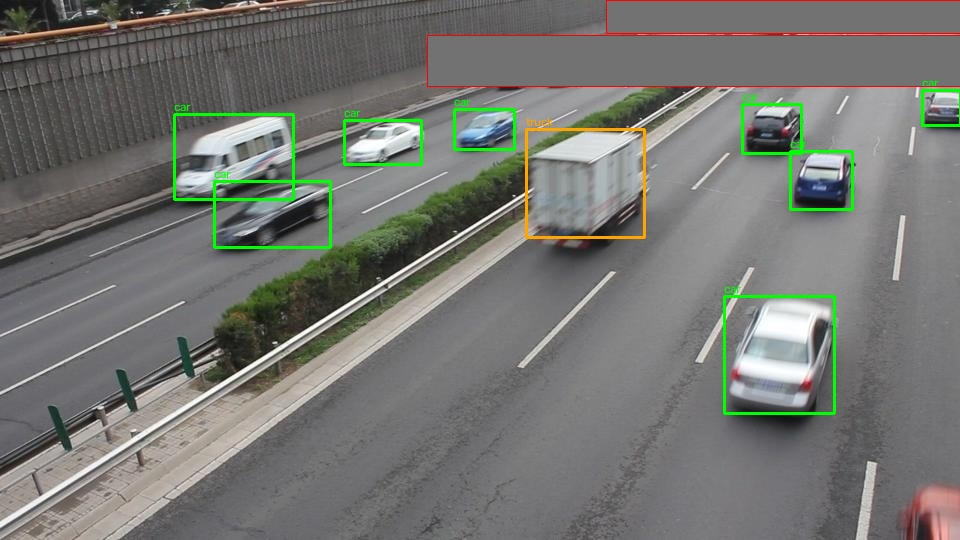
\includegraphics[width=0.8\linewidth]{hinh/detrac-train.jpg}
\caption{Ảnh huấn luyện UA-DETRAC, video MVI\_40241, khung 730, sau khi xuất nhãn mixed5. Hộp là nhãn dùng huấn luyện; các vùng xám đánh dấu phần bỏ qua. Nguồn ảnh và quy tắc chuyển đổi ở hồ sơ R52.}
\end{figure}
Phân bố lớp lệch mạnh về ô tô. Trong 476.062 hộp train, có 427.864 hộp ô tô nhưng chỉ có 2.235 hộp xe máy, đều thuộc BDD. UA-DETRAC không cung cấp nhãn riêng cho xe hai bánh. Một xe máy không có nhãn trong ảnh huấn luyện có thể trở thành ví dụ nền đối với detector. Vì thế, chất lượng ô tô không thể đại diện cho chất lượng xe máy. Nguồn nhãn train BDD là bản đóng gói lại đã ghim phiên bản và kiểm tra nội dung, chưa đối chiếu được với archive train gốc.

\section{Ba bộ phát hiện}
YOLOv8n COCO dùng trọng số gốc làm mốc. Hai detector còn lại, YOLOv8n mixed5 và YOLO11n mixed5, được khởi tạo từ trọng số COCO rồi huấn luyện 15 epoch trên tập trộn. Checkpoint dùng ở các vòng sau được chọn trên tập phát triển nội bộ, tương ứng epoch 15 và epoch 13. Đổi từ YOLOv8n COCO sang YOLOv8n mixed5 đồng thời đổi trọng số học được và không gian lớp. Điểm của cặp này đo kết quả của hai cấu hình hoàn chỉnh. Nó không cho biết mức cải thiện riêng do trộn thêm ảnh từ UA-DETRAC.

Đánh giá detector chạy FP32, kích thước danh nghĩa 640, ngưỡng thu nhận 0,001, NMS theo lớp ở IoU 0,7 và tối đa 300 hộp. Điểm precision và recall vận hành dùng ngưỡng 0,25. Đường tracking có cache riêng sinh ở ngưỡng 0,05. Với UA-DETRAC, đường sinh cache cho phép tới 3.000 hộp trước bước lọc lúc đọc để tránh cắt mất ứng viên sớm. Tên lớp của mô hình năm lớp được chuyển về ID COCO trước khi lọc. Hệ thống giữ thứ tự phát hiện sau NMS để các bộ lọc đối mặt với cùng bài toán gán.

\section{Cấu hình tracker và xử lý thời gian}
Hai điều kiện đầu vào được ký hiệu c25 và c10. Chúng giữ hộp có điểm lần lượt \emph{lớn hơn} 0,25 hoặc 0,10. ByteTrack giữ ngưỡng cao 0,25, ngưỡng thấp 0,10 và ngưỡng khởi tạo 0,25. Vòng ghép đầu dùng chi phí kết hợp IoU với điểm phát hiện, chấp nhận tới ngưỡng 0,8. Do đó ở c25, mọi hộp dưới ngưỡng cao đã bị loại từ đầu và vòng ghép điểm thấp rỗng. Ở c10, nhiều hộp có thể đi tiếp vào vòng này. Thêm ứng viên vừa có thể cứu một quỹ đạo vừa có thể tạo phép ghép sai, nên chênh lệch c10 và c25 cần đọc ở mức cấu hình.

Mỗi bộ lọc cung cấp cùng các thao tác khởi tạo, dự đoán và cập nhật. Cấu hình KF dùng trạng thái tám chiều. EKF và UKF dùng trạng thái chín chiều, cùng hàm chuyển CTRV và phép chiếu hộp. PF500 cơ sở dùng 500 hạt trên mỗi quỹ đạo, lấy mẫu lại theo ESS, tắt nhiễu bổ sung sau lấy mẫu lại và tắt đề xuất tối ưu. Hạt và bộ sinh ngẫu nhiên thuộc riêng từng quỹ đạo. Seed gốc cùng mã video và ID quyết định chuỗi số ngẫu nhiên. Ba seed 0, 1, 2 kiểm tra biến thiên khi chạy lại cùng cấu hình.

Biến thể PF500 K1/K2 dùng cho một số phép đối chiếu sau. K1 lấy mẫu lại các tọa độ quan sát từ phân bố Gauss điều kiện của từng hạt khi có phép đo. K2 thêm nhiễu sau lấy mẫu lại, với hệ số riêng cho phần hộp và phần chuyển động. Cấu hình motion2 nhân đôi hệ số nhiễu của nhóm biến chuyển động so với hệ số cơ sở của K2. Khi mất quan sát, bước dự đoán dựa vào trạng thái và nhiễu quá trình. Các bảng sau ghi rõ biến thể PF để tách các phép so với benchmark cơ sở.

Thời gian chờ khi mất dấu xấp xỉ 1,2 giây. Với UA-DETRAC ở 25 fps, giới hạn là 30 bước. Với BDD100K ở 5 fps, giới hạn chỉ còn 6 bước. Cùng hai bước liên tiếp ở hai tập tương ứng với hai khoảng thời gian vật lý khác nhau. Bộ lọc dự đoán theo bước ảnh và giữ đơn vị vận tốc theo bước. Khung hình không có phát hiện vẫn có vị trí trên trục thời gian theo giao thức của từng tập. Nếu loại các khung trống rồi đánh số liên tục lại, một khoảng mất quan sát sẽ bị rút ngắn giả tạo.

\subsection{Đề xuất có điều kiện đo trong PF}
Gọi $f_{ij}$ là tọa độ thứ $j$ sau mô hình chuyển của hạt $i$, $q_{ij}^2$ là phương sai quá trình theo tọa độ đó và $r_j^2$ là phương sai đo. Trong triển khai K1, bốn tọa độ $c_x,c_y,a,h$ có phép đo tuyến tính và nhiễu chéo. Phân bố dùng lấy mẫu tại những tọa độ này có phương sai và trung bình
\begin{align}
 s_{ij}^{2}&=\left(\frac{1}{q_{ij}^{2}}+\frac{1}{r_j^{2}}\right)^{-1},\\
 m_{ij}&=s_{ij}^{2}\left(\frac{f_{ij}}{q_{ij}^{2}}+\frac{z_j}{r_j^{2}}\right).
\end{align}
Sau đó $x_{ij}$ được lấy từ $\mathcal{N}(m_{ij},s_{ij}^2)$. Các tọa độ chuyển động tiếp tục dùng mẫu đã dự đoán. Hệ số cập nhật trọng số dựa vào mật độ dự đoán của phép đo, với log-mật độ bỏ hằng số chung
\[
 \ell_i=-\frac12\sum_{j\in\{c_x,c_y,a,h\}}
 \left[\frac{(z_j-f_{ij})^2}{q_{ij}^2+r_j^2}
       +\log(q_{ij}^2+r_j^2)\right].
\]
Phương sai quá trình phụ thuộc kích thước hộp từng hạt, nên số hạng log-phương sai được giữ. Thuật toán ép chiều cao dương sau lấy mẫu và chuẩn hóa trọng số trong miền log. Mục đích của K1 là sử dụng quan sát hiện tại khi đặt các mẫu ở phần trạng thái quan sát được, qua đó hạn chế tình trạng nhiều hạt được dự đoán ra xa phép đo. Hiệu quả giữ ID còn phụ thuộc việc tracker có ghép được phép đo cho quỹ đạo trước khi cập nhật.

\subsection{Theo dõi vòng đời và xử lý mất quan sát}
Mỗi quỹ đạo có thể đang hoạt động, đang mất dấu hoặc đã bị loại. Trong một khung, hệ thống thực hiện lần lượt các bước sau.
\begin{enumerate}
\item Giữ vị trí của khung trong dòng thời gian, đọc các phát hiện và lọc lớp, điểm theo giao thức.
\item Dự đoán trạng thái của các quỹ đạo thuộc nhóm được xét ghép.
\item Tính chi phí giữa hộp dự đoán và hộp quan sát, giải bài toán gán với ngưỡng của vòng đầu.
\item Thử ghép các quỹ đạo đang hoạt động còn đủ điều kiện với phát hiện điểm thấp, rồi xử lý quỹ đạo chưa được xác nhận.
\item Cập nhật bộ lọc ở các cặp ghép thành công, khởi tạo từ phát hiện còn lại đủ điểm, đánh dấu mất và loại những quỹ đạo hết thời gian chờ.
\item Ghi kết quả theo frame, ID và hộp trong hệ tọa độ ảnh gốc.
\end{enumerate}
Đối với khung thiếu phát hiện, dự đoán vẫn làm tăng tuổi mất dấu. Bộ lọc có thể đưa ra hộp dự báo trong khoảng này, còn quyết định ghi một quỹ đạo vào đầu ra do quy tắc vòng đời chi phối. Vì thế, cần kiểm cả bước bộ lọc lẫn việc quỹ đạo còn được xét ghép ở khung tái xuất hiện.

\section{Thiết kế phép so và kiểm tra tái lập}
Trong mỗi tập đánh giá chính, ba detector nhân hai ngưỡng nhân sáu lượt bộ lọc tạo thành 36 lượt. Sáu lượt gồm ba cấu hình xác định và ba seed PF500. Mỗi lượt đọc tất cả video của tập. Sau khi chấm COMBINED riêng cho từng seed, nghiên cứu lấy trung bình ba điểm PF. Việc này khác với trộn quỹ đạo của ba seed rồi chấm một lần. Một seed cho kết quả cao cũng không thay thế được kết quả trung bình.

Trên UA-DETRAC test40, mỗi checkpoint có 40 đơn vị cache. Hệ thống chấm đủ 1.440 đơn vị lượt--video. Trên BDD val, 600 đơn vị cache cung cấp đầu vào cho 7.200 đơn vị lượt--video. Phép kiểm tính lặp lại trên BDD gồm lặp tracker cho 36 lượt trên video định trước và chấm lại sáu lượt, đều trùng byte với đầu ra được đối chiếu. Các kiểm tra này xác nhận đường xử lý lặp lại được trong môi trường đã ghi nhận. Chúng không thay thế khoảng tin cậy cho biến thiên giữa video.

Đối với hiệu số trong một nhóm detector và ngưỡng, bootstrap lấy lại video theo cặp. Ở mỗi lần lấy mẫu, cùng danh sách chỉ số video được dùng cho hai bộ lọc, rồi tổ hợp lại các thành phần điểm. Cách làm này giữ quan hệ giữa các bộ lọc cùng gặp một video khó. Trên BDD, ma trận lấy mẫu gồm 5.000 lần, mỗi lần có 200 vị trí video. Trên UA-DETRAC, phân tích còn xét 39 nhóm để thử độ nhạy với một cặp video có liên hệ trong thiết kế phân nhóm. Các khoảng riêng lẻ không có hiệu chỉnh đa so sánh.

\section{Đường triển khai Jetson Nano}
Trên Nano, detector TensorRT nhận ảnh đã đổi kích thước và thêm đệm. Kết quả sau suy luận được lọc và đưa vào phiên bản tracker NumPy. Đường chạy trực tiếp vừa phát hiện vừa theo dõi. Đường phát lại dùng phát hiện đã lưu rồi chạy cùng tracker. So sánh tệp quỹ đạo giữa hai đường giúp phát hiện lỗi chuyển tọa độ, thứ tự hộp hoặc bước cập nhật ngay cả khi video hiển thị trông hợp lý.

Các phiên bản KF và EKF dùng backend NumPy trong phép đo đầu vào engine. Phép đo 80 video của cấu hình mới sử dụng KF trực tiếp trên Nano. Sau đó cache phát hiện từ cùng engine được chấm với cả bốn bộ lọc trên PC. Chương~\ref{chap:nano} trình bày các phép đo theo giai đoạn và điều kiện chạy của từng phép so.

\chapter{Thực nghiệm và thảo luận}
\section{Các tập đánh giá và đơn vị báo cáo}
\begin{table}[htbp]\centering\small
\caption{Phạm vi các phép đo tracking. Thời gian chờ được biểu diễn bằng số bước ở tốc độ của từng tập.}\label{tab:splits}
\begin{tabular}{lrrrl}\hline
Tập & Chuỗi & Khung hình & fps & Chờ\\\hline
UA-DETRAC test40 & 40 & 56.340 & 25 & 30 bước\\
BDD100K MOT val & 200 & 39.973 & 5 & 6 bước\\
SVMOT test & 9 & 8.250 & 30 & 36 bước\\
SVMOT bổ sung & 21 & 18.650 & 30 & 36 bước\\
RoundaboutHD phần đầu & 4 & 12.000 & 15 & 18 bước\\
RoundaboutHD phần mở rộng & 4 & 24.000 & 15 & 18 bước\\
Sherbrooke cars ROI & 1 & 1.001 & 30 & 36 bước\\
HELMET test & 182 & 18.200 & 10 & 12 bước\\
UTUAV B/C validation & 2 & 1.489 & 29,97 & 36 bước\\\hline
\end{tabular}
\end{table}
Trên UA-DETRAC, phép đo detector chỉ báo AP cho ô tô và xe buýt. Các vùng \emph{van}, \emph{others} và vùng bỏ qua không tham gia như nhãn dương của hai lớp đó. Có 173 ảnh thiếu phần tử khung hình trong XML nên còn 56.167 ảnh khi chấm detector. Trong phép đo tracking, bộ chấm dùng danh tính phương tiện gộp, kể cả \emph{van} và \emph{others}. Toàn bộ 56.340 ảnh vẫn đi qua đường theo dõi. Trên 173 ảnh nói trên, bộ chấm coi GT trống. Chưa đủ bằng chứng để coi mọi xe xuất hiện ở đó là phát hiện nhầm trong thế giới thực.

BDD val dùng nhãn COCO-video cho năm lớp và xử lý vùng crowd theo bộ chấm của dự án. Có 615 ảnh không có chú thích được giữ trong dòng thời gian. BDD val đã được quan sát trong quá trình phát triển, nên mức độ độc lập của tập này khác với một tập kiểm tra kín. SVMOT và RoundaboutHD chỉ có lần lượt hai cảnh và bốn camera của cùng một nút giao. Vì thế hai phép đánh giá ngoài chỉ báo kết quả mô tả. Một điểm HOTA cao hơn giữa hai tập có thể phản ánh quy tắc chấm, mật độ nhãn hoặc tốc độ lấy mẫu khác nhau.

HELMET được chấm trên toàn bộ test chính thức. Trong đó, 36 clip từng dùng để đánh giá ban đầu được đối chiếu lại và 146 clip còn lại được báo riêng để kiểm tra tính nhất quán. UTUAV được dùng để khảo sát giới hạn chuyển miền sang góc nhìn UAV trong hai block B và C. Các phép đo ngoài phục vụ những kịch bản riêng, với đơn vị nhãn và quy tắc đánh giá theo từng tập.

\section{Bộ phát hiện trước và sau tinh chỉnh}
\begin{table}[htbp]\centering\small
\caption{mAP của ba checkpoint trên thang 0--1. UA tính trên hai lớp, BDD tính trên năm lớp. Nguồn R53.}\label{tab:ap}
\begin{tabular}{lrrrr}\hline
& \multicolumn{2}{c}{UA-DETRAC test} & \multicolumn{2}{c}{BDD100K val}\\
Detector & 50 & 50--95 & 50 & 50--95\\\hline
YOLOv8n COCO & 0,8701 & 0,5997 & 0,2439 & 0,1571\\
YOLOv8n mixed5 & 0,8785 & 0,6111 & 0,3896 & 0,2544\\
YOLO11n mixed5 & 0,8884 & 0,6222 & 0,3787 & 0,2494\\\hline
\end{tabular}
\end{table}
Trên UA-DETRAC, YOLO11n mixed5 có mAP50 cao nhất trong ba checkpoint. Điểm trung bình che một khác biệt theo lớp. AP50 ô tô tăng từ 0,8577 ở YOLOv8n COCO lên 0,9055 ở YOLO11n mixed5, trong khi AP50 xe buýt giảm từ 0,8825 xuống 0,8713. Do đó, lựa chọn detector dựa trên mAP có thể khác lựa chọn của một ứng dụng chuyên theo dõi xe buýt.

Trên BDD val, YOLOv8n mixed5 cho mAP50 cao nhất. Đối với xe máy, AP50 tăng từ 0,1175 lên 0,2174 khi so hai cấu hình YOLOv8n. Dù vậy, recall vận hành của YOLOv8n mixed5 ở lớp xe máy chỉ đạt 0,2284 trên 902 hộp có nhãn, thấp hơn nhiều so với 0,7040 trên 341.436 hộp ô tô. Một bộ lọc phía sau detector chỉ có thể nối các quan sát thưa nếu quỹ đạo đã hình thành và thời gian chờ còn hiệu lực. Kết quả AP là ước lượng điểm; chưa có khoảng tin cậy AP cho test40 và BDD val.

Checkpoint YOLO11n 50/50 dùng trong phép đo Nano được kiểm tra riêng tại kích thước $384\times640$ trên PC. Trên BDD val, mô hình đạt mAP50 37,89\%, mAP50--95 24,74\% và AP50 xe máy 21,14\%. Trên UA-DETRAC test40, mAP50 của ô tô và xe buýt là 89,08\% và mAP50--95 là 62,40\%. Tương ứng, AP50 riêng của ô tô và xe buýt là 90,55\% và 87,60\%. Các điểm này đánh giá checkpoint 50/50 trên PC. Chất lượng tracking từ engine FP16 thực tế được chấm riêng trên các đoạn xử lý ở Chương~\ref{chap:nano}.

\begin{table}[htbp]\centering\small
\caption{Độ chính xác từng lớp của YOLO11n 50/50 trên BDD100K val. Các chỉ số theo phần trăm. Precision và recall ở ngưỡng vận hành 0,25. Nguồn R108.}\label{tab:ap-classes}
\begin{tabular}{lrrrrr}\toprule
Lớp & Hộp GT & AP50 & AP50--95 & Precision & Recall\\\midrule
Ô tô & 341.436 & 77,21 & 51,10 & 83,71 & 67,84\\
Xe tải & 27.343 & 37,62 & 26,74 & 70,25 & 31,40\\
Xe buýt & 9.087 & 36,74 & 27,95 & 58,97 & 34,47\\
Xe máy & 902 & 21,14 & 9,91 & 22,16 & 29,60\\
Xe đạp & 4.135 & 16,75 & 7,99 & 50,39 & 12,65\\\bottomrule
\end{tabular}
\end{table}
Độ lệch số lượng nhãn giữa các lớp đòi hỏi báo cáo AP riêng. Với checkpoint 50/50, lớp xe máy có recall cao hơn YOLO11n mixed5 ban đầu trong điểm vận hành đã đo, đồng thời precision thấp hơn. Điểm AP phản ánh nhiều ngưỡng điểm, còn một cấu hình tracking cụ thể chỉ nhận các hộp sau ngưỡng đã chọn. Chất lượng trên BDD vì vậy được báo cùng ma trận tracking khi detector bị cố định.

\section{Giữ ID khi cua và khi bị che}
Phép thử trên 12 video phát triển UA-DETRAC dùng YOLOv8n COCO ở ngưỡng trên 0,25. KF/CV đạt 59,00 HOTA, EKF 59,25 và UKF 58,79 trên thang 100. Khoảng tin cậy cho hiệu HOTA của từng cấu hình EKF và UKF so với CV đều chứa 0. PF100 đạt 49,33. Biến thể PF100 với phân bố đề xuất có dùng phép đo (K1) đạt 53,77. Đây là phép khảo sát trên tập phát triển với 100 hạt, tách biệt với benchmark 500 hạt ở các phần sau.

Phân tích che khuất bắt đầu với 717 sự kiện. Chỉ 184 sự kiện trên 137 quỹ đạo có đủ GT trước và sau để đánh giá việc nối ID. Trong 33 sự kiện che gần hoàn toàn trên sáu video, tỷ lệ giữ ID của các biến thể chỉ khoảng 0,02--0,09. Các khoảng tin cậy cho hiệu số đều chứa 0. Nếu tính cả trường hợp xe đã ra khỏi vùng có nhãn vào mẫu số, kết quả sẽ trộn mất ID với mất khả năng quan sát danh tính chuẩn.

Trong 1.185 quỹ đạo GT trên tập phát triển, tiêu chí dựa trên độ cong cực đại nhận được 32 quỹ đạo cua ở năm video. Khi dùng phân vị 90 thay cho cực đại, chỉ còn tám quỹ đạo ở bốn video. Tầng thứ hai chỉ dùng để đếm mẫu. Trên tầng thứ nhất, PF100 giữ ID kém hơn EKF. Không thể từ đây suy ra mô hình nào tốt nhất cho riêng xe máy rẽ. Cả nhãn loại xe lẫn số quỹ đạo cua có thể kiểm tra đều giới hạn câu trả lời.

\section{UA-DETRAC test40}
\begin{table}[htbp]\centering\small
\caption{HOTA COMBINED trên UA-DETRAC test40, thang 100. PF500 là trung bình điểm của ba seed. Nguồn R56.}\label{tab:ua}
\begin{tabular}{llrrrr}\hline
Detector & Ngưỡng & CV & EKF & UKF & PF500\\\hline
YOLOv8n COCO & c25 & 58,235 & 58,353 & 58,244 & 55,080\\
YOLOv8n COCO & c10 & 57,969 & 58,303 & 58,154 & 55,069\\
YOLOv8n mixed5 & c25 & 61,643 & 61,711 & 61,630 & 58,545\\
YOLOv8n mixed5 & c10 & 61,243 & 61,426 & 61,293 & 58,276\\
YOLO11n mixed5 & c25 & 62,063 & 62,239 & 62,181 & 58,811\\
YOLO11n mixed5 & c10 & 61,531 & 61,794 & 61,729 & 58,599\\
\hline\end{tabular}\end{table}

Đọc theo một hàng của Bảng~\ref{tab:ua} giữ được cùng phát hiện cho cả bốn bộ lọc. Trong nhóm YOLO11n mixed5 c25, EKF đạt 62,239 HOTA và CV đạt 62,063. Hiệu 0,176 điểm nhỏ hơn nhiều so với mức giảm khi thay CV bằng PF500 trong cùng nhóm. Khi giữ CV và đổi detector ở c25, điểm thay đổi từ 58,235 với YOLOv8n COCO lên 62,063 với YOLO11n mixed5. Phép so thứ hai cho thấy độ lớn của thay đổi cấu hình detector, nhưng thiết kế không có CI cho hiệu giữa detector.

Trên cả sáu hàng, độ chênh giữa CV, EKF và UKF tối đa 0,34 điểm HOTA. CI 95\% cho hiệu EKF trừ CV không chứa 0 ở hai trong sáu nhóm, gồm YOLOv8n COCO c10 và YOLO11n mixed5 c25. PF500 thấp hơn ba bộ lọc còn lại từ 2,90 đến 3,43 điểm HOTA trên các đối chứng của sáu nhóm. Các khoảng cho hiệu đó không chứa 0. Phân tích bootstrap được cố định sau khi đã xem điểm test40, nên các khoảng này có giá trị mô tả hậu nghiệm.

\subsection{Đối chứng với SORT}
Ở c25, sáu cặp cùng detector và cùng bộ lọc CV hoặc EKF cho HOTA ByteTrack cao hơn SORT từ 1,380 đến 3,714 điểm. Ví dụ với YOLOv8n COCO và CV, ByteTrack đạt 58,235 còn SORT đạt 54,521. IDSW giảm từ 4.318 xuống 2.498 nhưng FP tăng từ 62.846 lên 73.478. Trong cặp này, khả năng nối ID tốt hơn đi cùng nhiều hộp không khớp GT hơn. Chỉ số HOTA tổng hợp hai mặt của thay đổi đó.

Với YOLO11n mixed5 và CV, chênh HOTA chỉ còn 1,380 điểm. AssA tăng 2,921 điểm trong khi DetA giảm 0,060 điểm. Như vậy nguồn chênh chủ yếu nằm ở liên kết. Phép so chỉ thực hiện ở c25, nơi vòng ghép điểm thấp của ByteTrack rỗng. Khác biệt quan sát được thuộc về toàn bộ cơ chế ghép và quản lý vòng đời trong hai tracker. Không có CI cho sáu cặp này.

\section{BDD100K val}
\begin{table}[htbp]\centering\small
\caption{HOTA COMBINED trên BDD100K val, thang 100. PF500 là trung bình điểm của ba seed. Nguồn R61.}\label{tab:bdd}
\begin{tabular}{llrrrr}\hline
Detector & Ngưỡng & CV & EKF & UKF & PF500\\\hline
YOLOv8n COCO & c25 & 33,677 & 33,827 & 33,769 & 29,661\\
YOLOv8n COCO & c10 & 34,104 & 34,353 & 34,211 & 30,122\\
YOLOv8n mixed5 & c25 & 45,059 & 45,200 & 45,122 & 38,697\\
YOLOv8n mixed5 & c10 & 45,298 & 45,499 & 45,406 & 38,987\\
YOLO11n mixed5 & c25 & 44,856 & 45,061 & 44,955 & 38,620\\
YOLO11n mixed5 & c10 & 45,143 & 45,282 & 45,223 & 38,891\\
\hline\end{tabular}\end{table}

Điểm cao nhất trong ma trận thuộc YOLOv8n mixed5 c10 với EKF. Cấu hình này đạt HOTA 45,499, IDF1 55,170 và 11.067 lần đổi ID. So với CV trên cùng cache, hiệu HOTA là $+0{,}201$ điểm, CI 95\% từ $+0{,}081$ đến $+0{,}325$. Trong cùng nhóm, PF500 thấp hơn EKF 6,511 điểm với CI từ $-7{,}044$ đến $-5{,}980$. Hai cặp có độ lớn chênh rất khác nhau dù cùng được xét trên 200 video.

Trên cả sáu nhóm, EKF cao hơn CV về HOTA và sáu khoảng cho hiệu số đều nằm phía trên 0. Sáu khoảng UKF trừ CV đều chứa 0. PF500 thấp hơn các cấu hình còn lại về HOTA và IDF1 ở cả sáu nhóm. Việc chênh EKF và CV khá nhỏ nhưng khoảng nằm trên 0 trả lời câu hỏi về tính nhất quán trên mẫu video này. Mức chênh có đáng đổi cấu hình trong một ứng dụng cụ thể hay không còn phụ thuộc chi phí xử lý và yêu cầu về danh tính của ứng dụng.

\section{Chuyển sang cảnh và camera mới}
\subsection{SVMOT}
Bộ SVMOT có nhiều phương tiện dừng và nhiều trường hợp che khuất \cite{svmot}. Chín chuỗi test được ghi ở hai cảnh, bốn chuỗi buổi sáng và năm chuỗi buổi tối. Detector xử lý toàn ảnh theo giao thức dự án. Một xe xa nằm ngoài vùng có nhãn vẫn có thể bị tính FP. Ở c25 với YOLOv8n COCO, HOTA lần lượt là 48,66, 49,65, 49,21 và 50,70 cho CV, EKF, UKF và PF500. Tuy nhiên, khi tách theo cảnh, PF500 đạt 46,53 so với 46,78 của CV ở cảnh sáng, còn ở cảnh tối là 54,38 so với 50,39. Lợi thế tổng hợp của PF tập trung ở cảnh thứ hai. Chưa thể quy nguyên nhân cho ánh sáng vì cảnh quay và thời điểm thay đổi cùng nhau.

Ba seed PF500 trong nhóm này cho HOTA 51,30, 51,31 và 49,50. IDSW trung bình là 427,3 so với 407 của EKF. Có thể cải thiện HOTA dù còn nhiều lần đổi ID hơn vì HOTA cũng tính phát hiện và độ nhất quán liên kết trên toàn quỹ đạo. Với hai detector mixed5, DetA thấp hơn YOLOv8n COCO khoảng mười điểm. Không có CI trên hai cảnh và không dùng các điểm này để chọn lại checkpoint.

Phép kiểm che khuất gắn sự kiện với giá trị \emph{visibility} của hộp GT ở thời điểm đánh giá. Mức không quá 0,5 xác định nhóm che khuất trong Bảng~\ref{tab:svmot-vis}. Trong test chính thức, EKF có ít hơn KF mười lần đổi ID, còn UKF bằng KF. Trên 21 chuỗi thuộc split train chính thức, chiều chênh lệch đổi ID không lặp lại. Kết quả của 21 chuỗi được báo như một khảo sát mô tả riêng; điểm test chính thức giữ nguyên 9 chuỗi. Chênh lệch FN nhỏ trong từng nhóm cho phép đọc IDSW cùng với độ phủ mẫu.

\begin{table}[htbp]\centering\small
\caption{Kết quả SVMOT với YOLOv8n COCO c25 trên hai phần của bản phát hành.}\label{tab:svmot-vis}
\begin{tabularx}{\linewidth}{@{}Xrrrr@{}}\toprule
Phạm vi và chỉ số & Hộp GT & KF & EKF & UKF\\\midrule
9 chuỗi test, IDSW toàn phần & 70.220 & 435 & 407 & 418\\
9 chuỗi test, IDSW ở visibility $\leq0{,}5$ & 12.051 & 125 & 115 & 125\\
9 chuỗi test, FN ở visibility $\leq0{,}5$ & 12.051 & 6.515 & 6.517 & 6.497\\
21 chuỗi bổ sung, IDSW toàn phần & 173.242 & 1.189 & 1.162 & 1.162\\
21 chuỗi bổ sung, IDSW ở visibility $\leq0{,}5$ & 22.221 & 149 & 152 & 156\\
21 chuỗi bổ sung, FN ở visibility $\leq0{,}5$ & 22.221 & 12.637 & 12.630 & 12.626\\\bottomrule
\end{tabularx}
\end{table}

Trên test9, tỷ lệ hộp GT khả kiến thấp có ít nhất một phát hiện đạt IoU từ 0,5 tăng từ 49,03\% ở ngưỡng 0,25 lên 67,42\% ở ngưỡng 0,10. Đây là độ phủ ứng viên trước ghép một-một. Khi hạ ngưỡng, FN toàn video của KF giảm từ 14.665 xuống 12.924 và FP tăng từ 21.964 lên 29.836. Trong riêng nhóm đang che ở ngưỡng 0,10, IDSW là 105, 107 và 106 cho KF, EKF và UKF. Phép kiểm cho thấy sự đánh đổi giữa phục hồi quan sát và báo nhầm khi đưa thêm hộp vào ByteTrack.

\subsection{RoundaboutHD}
RoundaboutHD cung cấp nhãn cho cả bài toán đa camera và đơn camera \cite{round}. Giao thức lấy 3.000 khung liên tiếp đầu tiên của mỗi camera tại cùng một vòng xuyến. GT là quỹ đạo đơn camera trong SCT. Tám cặp hộp của ID 105 ở camera 4 trùng khóa khung--ID nhưng khác tọa độ. Quy trình bỏ cả 16 dòng liên quan ở các khung 2536--2543, giữ phần còn lại của quỹ đạo. Nhãn SCT không phủ các xe đỗ trong bãi. Một dự đoán đúng vị trí xe đỗ vẫn có thể bị tính FP. Quy tắc này ảnh hưởng trực tiếp đến cách diễn giải kết quả detector.

Với YOLOv8n mixed5 c25, CV đạt 42,83 HOTA, EKF đạt 42,48, UKF đạt 42,44 và PF500 chỉ đạt 31,27. Trên sáu nhóm, ba cấu hình đầu cách nhau tối đa 0,6 điểm. PF500 thấp hơn CV từ 11,56 đến 12,35 điểm ở COMBINED và có IDSW gấp 2,22 đến 2,91 lần. Chiều giảm xuất hiện trong đủ 72 tổ hợp camera, detector, ngưỡng và seed. Khác biệt này lớn hơn dao động giữa các seed. Bảng đầy đủ cho hai tập ngoài được trình bày ở Phụ lục~\ref{app:ho-so}.

\subsection{RoundaboutHD: đánh giá trên 24.000 khung tiếp theo}
Trong vòng mở rộng, mỗi camera dùng lại dự đoán detector của 3.000 khung đầu để tạo lịch sử tracker, rồi chạy tiếp đến khung 9.000. Bốn cấu hình dùng YOLOv8n COCO c25, chung giới hạn chờ 18 khung, với PF500 K1/K2 motion2 ở ba seed. Mốc rẽ được lấy từ GT trên toàn timeline. Tại mỗi khung, phương pháp lấy trung vị điểm giữa đáy hộp quanh ba mốc cách nhau 13 khung, rồi tính góc giữa hai vectơ dịch chuyển. Mỗi vectơ phải dài ít nhất $\max(8\,\text{px},0{,}25h)$, với $h$ là chiều cao hộp GT. Một đoạn rẽ yêu cầu ít nhất tám khung liên tiếp đạt ngưỡng và cùng chiều đổi hướng. Ngưỡng chính là $25^\circ$, ngưỡng $35^\circ$ dùng để kiểm tra độ nhạy, còn nhóm gần thẳng dùng tối đa $8^\circ$. Góc được đo trên ảnh và chịu ảnh hưởng của phối cảnh.

\begin{table}[htbp]\centering\small
\caption{Số lần đổi ID theo nhóm chuyển động trên phần mở rộng RoundaboutHD. PF là trung bình ba seed.}\label{tab:round-ext}
\begin{tabular}{@{}lrrrrr@{}}\toprule
Nhóm & Hộp GT & KF & EKF & UKF & PF500\\\midrule
Đổi hướng từ $25^\circ$ & 13.509 & 34 & 28 & 28 & 40,33\\
Đổi hướng từ $35^\circ$ & 8.659 & 29 & 24 & 24 & 33,00\\
Gần thẳng & 78.372 & 426 & 423 & 418 & 658,67\\
Toàn cửa sổ mới & 157.222 & 716 & 726 & 725 & 1.020,33\\\bottomrule
\end{tabular}
\end{table}
Với ngưỡng $25^\circ$, EKF và UKF cùng giảm 17,65\% IDSW so với KF. Số lượt bỏ sót tương ứng của KF, EKF và UKF là 5.275, 5.264 và 5.263. Mức giảm IDSW xuất hiện trên camera 1, 2 và 3. Ở camera 4, cả ba cấu hình đều có 10 lần đổi ID trong nhóm này. Khi xét từng đoạn, 645 trong 652 đoạn có cùng số lần đổi ID giữa ba bộ lọc. Cả EKF và UKF cùng cải thiện ở sáu đoạn và cùng tăng IDSW ở một đoạn. Hình~\ref{fig:trajectory-cases} minh họa một trường hợp của mỗi chiều thay đổi.

\begin{figure}[htbp]\centering
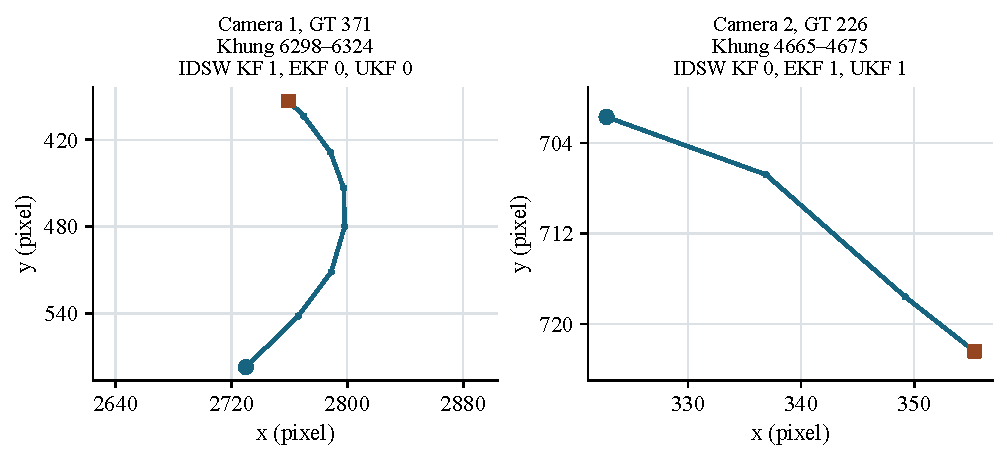
\includegraphics[width=\linewidth]{hinh/quy-dao-roundabout.pdf}
\caption{Hai đoạn đổi hướng trên RoundaboutHD. Đường biểu diễn tâm đáy hộp GT trên ảnh, với dấu tròn ở đầu và dấu vuông ở cuối. Hai ví dụ được chọn sau khi chấm để minh họa các trường hợp trái chiều.}\label{fig:trajectory-cases}
\end{figure}

Khi chấm toàn bộ 24.000 khung mới, KF có IDSW thấp nhất và HOTA cao nhất, 40,46\%. HOTA tương ứng của EKF, UKF và PF500 là 40,37\%, 40,19\% và 37,33\%. Kết quả theo nhóm rẽ mô tả các sự kiện được ghi trong lịch sử ghép liên tục. Điểm gộp toàn cửa sổ được chấm với lịch sử đánh giá bắt đầu ở khung 3.001, nên có thể lệch vài sự kiện ngay ranh giới. Toàn bộ bốn góc quay thuộc cùng một vòng xuyến. Điều này giới hạn khả năng suy rộng tỷ lệ giảm sang các nút giao độc lập.

\subsection{HELMET: theo dõi xe máy trên toàn tập test}
Tập HELMET cung cấp chuỗi phương tiện hai bánh ở 12 nhóm cảnh \cite{helmet}. Tập test chính thức chứa 182 clip, 18.200 khung, 54.529 hộp GT và 1.788 ID tính theo clip. Bộ lọc được so trên cùng cache YOLO11n mixed5 ở c10. Tại IoU 0,50 và ngưỡng điểm lớn hơn 0,10, detector đạt precision 45,17\% và recall 42,38\% cho xe máy. Hộp GT thường bao cả xe và người ngồi. Kết quả theo dõi phản ánh toàn clip theo quy tắc chú thích đó.

\begin{table}[htbp]\centering\small
\caption{So sánh trên HELMET với YOLO11n mixed5 c10. PF500 là trung bình ba seed.}\label{tab:helmet}
\begin{tabular}{@{}lrrrr@{}}\toprule
Phạm vi và chỉ số & KF & EKF & UKF & PF500\\\midrule
182 clip, IDSW & 717 & 444 & 452 & 630\\
182 clip, HOTA (\%) & 20,81 & 21,66 & 21,82 & 18,71\\
146 clip bổ sung, IDSW & 639 & 390 & 398 & 554,33\\
146 clip bổ sung, HOTA (\%) & 21,22 & 22,13 & 22,21 & 19,12\\\bottomrule
\end{tabular}
\end{table}
Trên toàn tập test, EKF giảm 38,08\% IDSW và UKF giảm 36,96\% so với KF, đồng thời HOTA tăng trên cả hai cấu hình. Mức giảm IDSW vẫn xuất hiện khi tách riêng 146 clip chưa dùng trong lượt test36. Số FN của cả bốn cấu hình còn cao, từ 43.644 đến 44.813 tùy lượt. Vì chưa phân tầng HELMET theo lúc xe đổi hướng hoặc che khuất, phép đo này hỗ trợ nhận định về giữ ID xe máy trên tập test mà chưa tách được tác động của từng kịch bản.

\subsection{UA-DETRAC: đổi ID ở các đoạn che khuất}
Phép hậu kiểm R113 dùng 40 đoạn test, mỗi đoạn 150 khung, với cùng phát hiện YOLO11n 50/50 c25 từ Jetson Nano. Mỗi lần đổi ID và mỗi hộp bỏ sót được quy về hộp GT tại khung đó sau khi phát lại lịch sử ghép CLEAR trên toàn đoạn. Phép kiểm khớp tổng IDSW và FN ở cả 120 tổ hợp đoạn và bộ lọc.

\begin{table}[htbp]\centering\small
\caption{Kết quả theo khả kiến trên 40 đoạn UA-DETRAC. Trong mỗi ô là IDSW và FN, theo thứ tự.}\label{tab:ua-occlusion-r113}
\begin{tabular}{@{}lrrrr@{}}\toprule
Phạm vi & Hộp GT & KF & EKF & UKF\\\midrule
Khả kiến $\leq 0{,}5$ & 7.486 & 53 / 4.941 & 50 / 4.940 & 48 / 4.939\\
Có che trong một giây gần nhất & 10.097 & 86 / 5.793 & 83 / 5.792 & 77 / 5.791\\
Toàn đoạn & 74.354 & 245 / 17.590 & 250 / 17.593 & 248 / 17.591\\\bottomrule
\end{tabular}
\end{table}

Trong 7.486 hộp có khả kiến thấp, EKF giảm 5,66\% và UKF giảm 9,43\% IDSW so với KF, với chênh lệch tối đa hai hộp bỏ sót. Bootstrap ghép cặp theo 40 đoạn cho khoảng phân vị 95\% của chênh lệch IDSW là $[-8,2]$ với EKF và $[-15,3]$ với UKF. Cả hai khoảng đều chứa 0. Kết quả toàn đoạn cho thứ hạng khác. Nhóm gồm xe vừa rẽ từ $25^\circ$ vừa bị che chỉ có 34 hộp, trong đó mỗi bộ lọc bỏ sót 32 hộp. Cần thêm dữ liệu hỗn hợp để kiểm chứng đồng thời xe rẽ, xe bị che và từng loại phương tiện.

\subsection{Đối chiếu đổi hướng với camera gắn xe}
Trên 40 đoạn BDD100K, nhóm đổi hướng trên ảnh từ $25^\circ$ có 2.205 hộp xe. IDSW lần lượt là 64, 61 và 59 với KF, EKF và UKF. Riêng ô tô có 1.896 hộp và IDSW 58, 56 và 54. Số bỏ sót ô tô lần lượt là 973, 977 và 978. 147 hộp xe máy trong mẫu chưa tạo đoạn đạt tiêu chí rẽ. Đây là phân nhóm theo lớp GT của phép ghép phương tiện gộp.

Hai clip METEOR \cite{meteor} được chọn theo số đoạn đổi hướng trong nhãn trước khi xem kết quả. Trong nhóm rẽ có 425 hộp ô tô và 670 hộp xe máy hoặc scooter. IDSW ô tô bằng 0 ở cả ba bộ lọc, với 294 hộp bỏ sót mỗi bộ lọc. IDSW xe máy là 2, 1 và 1, với 658 hộp bỏ sót mỗi bộ lọc. Chỉ 18 hộp xe máy rẽ có phát hiện cùng lớp đạt IoU ít nhất 0,5. Độ phủ thấp và số lần đổi ID ít giới hạn giá trị suy rộng của pilot. Cả BDD và METEOR đều đo đổi hướng trên ảnh, nên kết quả bao hàm chuyển động của camera.

\section{Chẩn đoán sai số PF trên RoundaboutHD}
Để tìm chênh lệch xuất hiện ở bước nào, nghiên cứu cố định YOLOv8n mixed5 c25 và ghi trạng thái ngay sau dự đoán, trước ghép. Với mỗi cấu hình và camera, hai đường bật và tắt ghi log phải trả cùng quỹ đạo. Cả 24 đơn vị đều trùng byte với kết quả benchmark. Các chuỗi kiểm tra trạng thái nội bộ sau dự đoán, cập nhật và các bước PF cũng trùng giữa hai đường.

Phép chẩn đoán nối đầu ra ở quan sát trước với GT bằng phép ghép một-một, loại ứng viên IoU dưới 0,5 trước khi gán, rồi theo cùng GT tới khung hiện tại. Sai số là khoảng cách tâm dự đoán đến tâm GT chia cho chiều cao hộp GT. Khoảng hai khung có chỉ số cách nhau một đơn vị tương ứng với \emph{không} có khung thiếu quan sát ở giữa. Trên 35.465 bộ camera--ID chuẩn--khung liền kề hợp lệ ở cả sáu lượt, sai số trung vị của CV là 0,063 chiều cao hộp, PF là 0,095--0,096. IoU trung vị tương ứng là 0,810 và 0,739--0,742.

\begin{table}[htbp]\centering\small
\caption{Sai số tâm trung vị theo số khung thiếu quan sát. Số đo tính trên mẫu nối được GT của từng bộ lọc. Khoảng PF là min--max của ba seed. Nguồn R65, lượt chẩn đoán thứ hai.}\label{tab:gap}
\begin{tabular}{lrrrr}\hline
Bộ lọc & 0 & 1--2 & 3--8 & Ít nhất 9\\\hline
CV & 0,063 & 0,122 & 0,274 & 0,80\\
EKF & 0,060 & 0,113 & 0,266 & 0,86\\
UKF & 0,060 & 0,114 & 0,269 & 0,86\\
PF500 & 0,097--0,098 & 0,174--0,179 & 0,524--0,533 & 1,58--1,65\\\hline
\end{tabular}
\end{table}

\begin{figure}[htbp]\centering\small
\begin{tabular}{lcll}\hline
Khung thiếu & Bộ lọc & Sai số tâm / chiều cao hộp GT & Trung vị\\\hline
0 & CV & \rule{2.52mm}{1.6mm} & 0,063\\
  & PF & \rule{3.92mm}{1.6mm} & 0,098\\[2pt]
1--2 & CV & \rule{4.88mm}{1.6mm} & 0,122\\
  & PF & \rule{6.96mm}{1.6mm} & 0,174\\[2pt]
3--8 & CV & \rule{10.96mm}{1.6mm} & 0,274\\
  & PF & \rule{21.32mm}{1.6mm} & 0,533\\[2pt]
$\geq9$ & CV & \rule{32mm}{1.6mm} & 0,80\\
  & PF & \rule{66mm}{1.6mm} & 1,65\\\hline
\end{tabular}
\caption{Sai số dự đoán trên RoundaboutHD với YOLOv8n mixed5 c25. Độ dài thanh biểu diễn trung vị trên mẫu nối được GT của mỗi bộ lọc. PF dùng seed 0. Các nhóm có thành phần mẫu khác nhau.}
\end{figure}

Ở nhóm thiếu từ ba đến tám khung, sai số PF đã xấp xỉ nửa chiều cao hộp. Trên toàn bộ mẫu hợp lệ của mỗi cấu hình, tỷ lệ có phát hiện phù hợp với GT nhưng chi phí ghép không đạt là 8,63--8,83\% với PF và 3,68\% với CV. Tỷ lệ có ứng viên khả thi nhưng ứng viên bị quỹ đạo khác lấy chỉ là 0,68--0,75\% với PF và 0,89\% với CV. Hai nhóm thất bại này có ý nghĩa khác nhau. Nhóm đầu cho thấy có xe đúng trong đầu vào nhưng hộp dự đoán và điểm phát hiện chưa đủ cho phép gán. Nhóm sau mới phản ánh cạnh tranh giữa quỹ đạo. Phần lớn mức tăng ở nhóm đầu thuộc quỹ đạo đã mất dấu.

Trên 352 ID chuẩn, số lần phân mảnh tăng từ 1.944 ở CV lên 2.262--2.323 ở PF. Số quỹ đạo được theo dõi phần lớn thời gian giảm từ 79 xuống còn 46--48. Trung vị $N_{\mathrm{eff}}/N$ trước lấy mẫu lại là 0,188 và ngưỡng 0,5 bị vượt theo chiều giảm ở gần như mọi lần cập nhật. Khi thiếu ít nhất ba khung, sai số tâm tăng nhanh hơn độ trải hạt. Đây là các quan sát cùng xuất hiện. Phép thử không thay độc lập từng yếu tố như nhiễu, số hạt hay tốc độ khung nên nguyên nhân của sự giảm điểm vẫn chưa xác định. PF còn có nhiều mẫu không nối được GT hơn CV, vì vậy sai số trên các mẫu hợp lệ có thể đánh giá thấp mức khó của PF.

\section{Đối chiếu PF với triển khai công khai}
Thư viện Python \texttt{pfilter} phiên bản 0.2.5 cung cấp một triển khai lấy mẫu quan trọng và lấy mẫu lại (SIR) \cite{pfilter}. Phép thử đưa triển khai này vào cùng bộ nối ByteTrack và giữ số hạt, CTRV, cache, phép đo và dữ liệu chấm của cấu hình PF500 K1/K2 motion2. Hai nhánh khác nhau ở cách xây dựng đề xuất từ phép đo, bước lấy mẫu lại và xử lý các tình huống suy biến. Do các chi tiết này thay đổi cùng nhau, phép đối chứng đánh giá toàn bộ cách cập nhật hạt đã tích hợp.

\begin{table}[htbp]\centering\small
\caption{Đối chiếu hai triển khai PF trên 12 clip UA-DETRAC phát triển. Giá trị là trung bình ba seed. Nguồn R108.}\label{tab:pf-public}
\begin{tabular}{lrrrr}\toprule
Cấu hình & HOTA (\%) & IDF1 (\%) & IDSW & FN\\\midrule
PF500 K1/K2 motion2 & 57,01 & 68,36 & 697,00 & 39.395,67\\
PF500 với \texttt{pfilter} & 52,68 & 60,54 & 1.359,33 & 42.983,67\\\bottomrule
\end{tabular}
\end{table}

IDSW tăng ở cả ba seed với triển khai công khai. Khóa luận giữ PF500 K1/K2 motion2 cho các phép đối chiếu gần nhất. Biến thể ghép lại quỹ đạo Lost bằng IoU trong ba khung từng giảm IDSW từ 697 xuống 525,7 trên UA-DETRAC phát triển. Khi áp dụng lên BDD val, IDSW trung bình tăng từ 6.291,3 lên 6.712,3. Khoảng ba khung tương ứng 0,12 giây ở UA-DETRAC và 0,60 giây ở BDD, có thể góp phần vào thay đổi nhưng chưa được tách thành phép kiểm riêng. Biến thể ghép lại này không được chọn cho cấu hình chính.

\section{UTUAV và giới hạn của đầu vào}
UTUAV có cảnh giao thông nhìn từ trên cao và nhãn xe máy \cite{utuav}. Phép thử dùng hai block validation B gồm 738 khung và C gồm 751 khung. Tác giả xác nhận qua thư riêng rằng video B/C có tốc độ $30000/1001$ fps và ảnh được lấy liên tiếp với stride 1. Bước thời gian là $1001/30000$ giây và bộ đệm 1,2 giây tương ứng 36 bước.

Toàn bộ 36 lượt tracking cho ba detector, hai ngưỡng và sáu lượt bộ lọc đã hoàn tất. YOLOv8n COCO có độ phủ cao nhất, nhưng cận trên recall ở IoU 0,5 và conf $>0{,}05$ chỉ là 520/29.756 hộp GT động tại B (1,75\%) và 1.107/125.005 tại C (0,89\%). Phép kiểm này không buộc ghép một-một nên chỉ dùng làm cận trên độ phủ. HOTA của mọi cấu hình không vượt 0,46 trên thang 100.

Phát hiện quá thưa hạn chế khả năng phân biệt bộ lọc. Trường \texttt{occluded} trong nhãn đều bằng 0 nên chưa dùng để phân tầng che khuất. Kết quả này cho biết giới hạn chuyển miền của ba detector trong giao thức đã chạy.




\chapter{Tối ưu và đo kiểm trên Jetson Nano}\label{chap:nano}
\section{Từ checkpoint đến chương trình chạy trên thiết bị}
Checkpoint YOLO lưu tham số của mạng. Khi xuất ONNX, chương trình ghi kiến trúc và trọng số đã học thành một đồ thị phục vụ suy luận. TensorRT đọc đồ thị, chọn cách triển khai từng phép toán cho GPU và xây dựng engine cho kích thước đầu vào đã định \cite{tensorrt}. Lúc xử lý video, ảnh đã giải mã được thu nhỏ, đệm để giữ tỷ lệ, đổi thứ tự kênh và chuẩn hóa rồi mới ghi vào tensor. Engine nhận tensor đó để suy luận. Hộp dự đoán được đổi về tọa độ ảnh gốc trước khi loại hộp trùng và đưa vào ByteTrack.

\section{Định nghĩa thông lượng và độ trễ}
Gọi $T$ là thời gian xử lý cửa sổ gồm $n$ khung sau giai đoạn làm nóng. Thông lượng được tính theo $n/T$. Độ trễ của khung $i$ được tính theo chênh lệch timestamp lúc tracker hoàn tất với lúc bắt đầu đọc ảnh đó. Trong đường tuần tự, thời gian một khung gồm đọc và giải mã, tiền xử lý, sao chép tensor, chạy engine, hậu xử lý và cập nhật tracker. Khi gối đầu giải mã với suy luận, tổng thời gian các công đoạn của một ảnh có thể vượt khoảng cách giữa hai khung hoàn tất.

Với hai công đoạn có thời gian ổn định $t_1,t_2$, mô hình lý tưởng của đường tuần tự cần $t_1+t_2$ cho mỗi ảnh. Đường gối đầu sau khi làm đầy có thể hoàn tất một ảnh sau khoảng $\max(t_1,t_2)$, nhưng vẫn mất ít nhất $t_1+t_2$ để đưa một ảnh qua cả hai công đoạn. Chi phí đồng bộ, băng thông dùng chung và hàng chờ làm thời gian thực tế khác mô hình lý tưởng. Cách đo trong khóa luận giữ timestamp ở từng khung để đọc FPS cùng p90 độ trễ. Giá trị FPS trung bình theo video và FPS từ tổng khung chia tổng thời gian đều được kiểm tra trong hồ sơ R109.

\section{Giảm chi phí suy luận và sao chép}
Đổi kích thước đầu vào từ $640\times640$ sang $384\times640$ (cao $\times$ rộng) giảm 40\% số vị trí điểm ảnh trong tensor. Với ảnh ngang $960\times540$, hệ số co theo chiều rộng là $640/960$. Phần ảnh sau thu nhỏ là $640\times360$. Engine vuông cần thêm 280 hàng đệm, còn engine chữ nhật cần 24 hàng. Mạng tích chập vẫn xử lý cả vùng đệm, nên tổng số vị trí cần tính giảm khi dựng engine chữ nhật. Trọng số YOLO được giữ trong phép đối chứng kích thước.

\begin{table}[htbp]\centering
\caption{Đầu vào vuông và chữ nhật trên Nano. Thời gian GPU đo riêng cho engine, FPS lấy trung vị theo cấu hình trong phép thử R63.}\label{tab:nano}
\begin{tabular}{lrr}\toprule
Đại lượng & $640\times640$ & $384\times640$\\\midrule
Thực thi GPU của engine (ms) & 68,11 & 41,86\\
Toàn hệ thống với KF (FPS) & 9,27 & 13,24\\
Toàn hệ thống với EKF (FPS) & 9,23 & 13,20\\\bottomrule
\end{tabular}
\end{table}
R63 chạy 300 ảnh JPEG của MVI\_39031 mỗi lượt trên Nano 4 GB, chế độ MAXN, TensorRT 8.2 FP16 và bật HDMI. Trong năm cặp có thời gian giải mã cùng mức, cấu hình chữ nhật tăng FPS 42--44\%. Độ chính xác được đối chiếu riêng. Trên UA-DETRAC test40 tại c25, HOTA của KF và EKF tăng 0,09 và 0,20 điểm, trong khi recall xe nhỏ và xe che nặng giảm 0,60 và 0,81 điểm. Trên BDD val, HOTA giảm 0,02 điểm cho mỗi bộ lọc, recall xe nhỏ giảm 0,18 điểm.

Cấu hình v21combo dùng bảng 256 phần tử để chuẩn hóa giá trị pixel $u$ theo $u/255$ và giảm sao chép bộ đệm đầu ra. Bảng được tính một lần theo kiểu số của tensor, sau đó mỗi giá trị màu nguyên dùng trực tiếp làm chỉ số tra. Ở cùng engine chữ nhật, hai thay đổi cùng tăng FPS ghép cặp 5,39\% với KF và 5,12\% với EKF trên bài đo HDMI R83. Phép đo nhiều video R86 so v16 với v21combo trên 40 video mỗi tập. Trung vị mức tăng theo video của KF là 51,96\% ở BDD và 52,38\% ở UA-DETRAC. Mức tăng tương ứng của EKF đều là 47,74\%. 

\section{Cấu hình hướng tới 15 FPS}
Cấu hình R109 giữ engine FP16 $384\times640$ và thay checkpoint bằng YOLO11n 50/50. Hai checkpoint có cùng kiến trúc, gồm mixed5 và nhánh tinh chỉnh trên RideSafe. Tham số cùng vị trí được lấy trung bình với trọng số bằng nhau. Phép chấm riêng detector được báo ở Chương~4. Hệ thống còn loại hộp dưới ngưỡng 0,25 trước NMS, tính IoU bằng các phép toán mảng trong NMS và giải mã JPEG của khung kế tiếp song song với xử lý khung hiện tại. Kết quả được đưa vào tracker đúng thứ tự khung. Với ngưỡng đầu vào 0,25 của giao thức này, phép so dành cho nhánh c25. Nhánh c10 vẫn cần giữ các phát hiện điểm thấp hơn.

Để kiểm tác động riêng của giải mã gối đầu, R108 giữ detector và NMS trên 16 đoạn. Kết quả MOT và lớp khớp từng byte với đường xử lý tuần tự. Mức tăng FPS ghép cặp là 31,55\% ở BDD và 16,54\% ở UA-DETRAC. Ở R109, so sánh bao gồm cả thay checkpoint và thay cách xử lý. Lợi ích của từng thành phần vì vậy được đối chiếu bằng phép thử kiểm soát tương ứng.

\section{Kết quả trên 80 đoạn video}
Mỗi tập có 40 video, mỗi video lấy 150 ảnh JPEG liên tiếp theo manifest R86. Hai cấu hình đọc cùng ảnh từ tmpfs, dùng ByteTrack KF c25, tắt hiển thị và đảo thứ tự chạy qua các video. FPS tính trên cửa sổ ổn định bỏ 25 khung đầu. Cả 160 lượt đều xử lý đủ khung, tương ứng 24.000 lượt suy luận. Số đo gộp dưới đây là trung bình FPS theo video, với hai tập có số video bằng nhau.

\begin{figure}[htbp]\centering
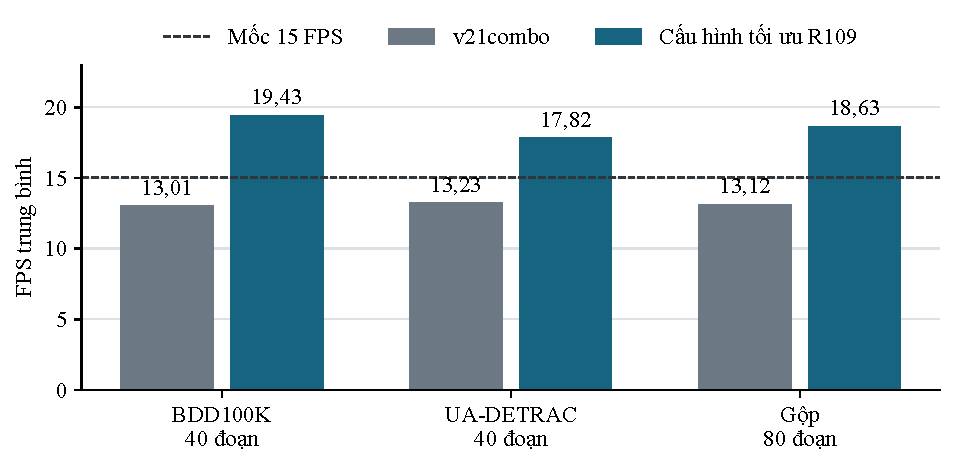
\includegraphics[width=.88\linewidth]{hinh/fps-jetson-nano.pdf}
\caption{FPS trung bình trên Jetson Nano. Hai cấu hình đọc cùng 80 đoạn JPEG và dùng KF. Đường đứt biểu thị mốc 15 FPS. Nguồn R109.}\label{fig:fps-nano}
\end{figure}

Trung bình tăng từ 13,12 lên 18,63 FPS, tương đương 41,99\%. BDD tăng 49,35\% và UA-DETRAC tăng 34,76\%. Bản tối ưu nhanh hơn trên cả 80 đoạn, đạt ít nhất 15 FPS ở 80/80 đoạn và có giá trị thấp nhất 16,66 FPS. Trung vị p90 theo video tăng từ 90,08 lên 123,88 ms. FPS đo số khung hoàn tất trên một đơn vị thời gian. Độ trễ tại đây tính từ khi bắt đầu đọc một ảnh đến khi tracker xử lý xong, gồm thời gian chờ sau giải mã. Hai khung ở hai công đoạn khác nhau có thể được xử lý cùng lúc, nên thông lượng tăng trong khi một ảnh mất thêm thời gian qua toàn chuỗi.

\begin{table}[htbp]\centering\small
\caption{Chất lượng tracking của hai cấu hình Jetson Nano với KF. HOTA, IDF1 tính theo phần trăm. Nguồn R109.}\label{tab:nano-quality}
\begin{tabular}{llrrrr}\toprule
Tập & Cấu hình & HOTA & IDF1 & IDSW & FN\\\midrule
BDD100K & v21combo & 33,51 & 38,96 & 971 & 37.403\\
 & R109 & 43,72 & 52,97 & 1.534 & 28.539\\
UA-DETRAC & v21combo & 62,81 & 73,72 & 280 & 22.287\\
 & R109 & 66,57 & 78,37 & 245 & 17.590\\\bottomrule
\end{tabular}
\end{table}

Bảng~\ref{tab:nano-quality} cho thấy HOTA và IDF1 tăng ở cả hai tập, đồng thời số hộp bỏ sót giảm. IDSW tăng ở BDD và giảm ở UA-DETRAC. So sánh hai cấu hình thay detector nên các tập xe được ghép và số cơ hội xảy ra đổi ID cũng thay đổi. Để đánh giá ảnh hưởng của bộ lọc, R110 lưu một lần detection từ engine Nano mới rồi phát lại trên PC với cùng cutoff, ánh xạ lớp, bước thời gian và đệm 1,2 giây. Đầu ra KF phát lại khớp số đo theo video của R109. Bảng~\ref{tab:nano-filters} trình bày kết quả khi đầu vào đã được cố định.

\begin{table}[htbp]\centering\small
\caption{Bộ lọc dùng cùng detection của Nano, phát lại trên PC. HOTA theo phần trăm. PF500 và RBPF500 báo trung bình ba seed. Nguồn R110 và R113.}\label{tab:nano-filters}
\begin{tabular}{lrrrr}\toprule
 & \multicolumn{2}{c}{BDD100K} & \multicolumn{2}{c}{UA-DETRAC}\\
Bộ lọc & HOTA & IDSW & HOTA & IDSW\\\midrule
KF & 43,72 & 1.534 & 66,57 & 245\\
EKF & 43,87 & 1.354 & 66,59 & 250\\
UKF & 43,74 & 1.426 & 66,61 & 248\\
PF500 K1/K2 & 42,81 & 1.569,67 & 65,94 & 276,33\\
RBPF500 & 43,60 & 1.450,33 & 66,69 & 246,33\\\bottomrule
\end{tabular}
\end{table}

So với KF, EKF giảm 11,73\% IDSW và UKF giảm 7,04\% ở BDD. KF có IDSW thấp nhất ở UA-DETRAC, nơi chênh giữa ba bộ lọc Kalman chỉ từ ba đến năm lần đổi ID. RBPF500 giảm IDSW so với PF500 K1/K2 7,60\% ở BDD và 10,86\% ở UA-DETRAC, đồng thời tăng HOTA ở cả hai tập. RBPF lấy mẫu hướng và tốc độ quay, còn bảy thành phần dùng Gaussian điều kiện cho từng hạt theo nguyên lý Rao--Blackwell \cite{doucet_rbpf}. Đây là kết quả chất lượng phát lại trên PC.

\section{Thông lượng và độ trễ của từng bộ lọc trên Nano}
R114 dùng tám đoạn BDD100K và tám đoạn UA-DETRAC, lấy cách đều từ hai nhóm 40 đoạn đã chọn ở R109. Bốn bộ lọc chạy trên cùng engine và 150 ảnh JPEG của từng đoạn, không bật hiển thị. Mỗi lượt giữ nguyên bước thời gian, ngưỡng ghép và thứ tự khung; thứ tự chạy bộ lọc được luân phiên giữa các đoạn. RBPF500 dùng seed 0. FPS và p90 lấy trên 125 khung sau 25 khung làm nóng. Phép đo tách thời gian khởi tạo engine khỏi FPS ổn định.

\begin{table}[htbp]\centering\small
\caption{Tốc độ trên Jetson Nano theo bộ lọc. FPS là trung bình theo đoạn. P90 là trung vị độ trễ p90 theo đoạn, đơn vị ms.}\label{tab:nano-r114}
\begin{tabular}{@{}lrrrrrr@{}}\toprule
 & \multicolumn{3}{c}{BDD100K} & \multicolumn{3}{c}{UA-DETRAC}\\
Bộ lọc & FPS & P90 & Đạt 15 FPS & FPS & P90 & Đạt 15 FPS\\\midrule
KF & 19,60 & 115,5 & 8/8 & 18,01 & 124,0 & 8/8\\
EKF & 19,61 & 116,1 & 8/8 & 18,04 & 127,8 & 8/8\\
UKF & 19,62 & 130,3 & 8/8 & 16,39 & 146,7 & 6/8\\
RBPF500 & 13,80 & 611,9 & 4/8 & 8,68 & 911,5 & 2/8\\\bottomrule
\end{tabular}
\end{table}

Trong 64 lượt, detector suy luận đủ 9.600 khung, với cache trùng từng byte phiên bản R110 tương ứng. 16 lượt KF trùng byte kết quả MOT và lớp của R109. Đầu ra MOT của cả 64 lượt khớp lần phát lại trên PC về ID, khung và điểm số, với sai số tọa độ tối đa cho phép $10^{-3}$ px. KF và EKF đạt 15 FPS ở cả 16 đoạn. UKF đạt ở 14 đoạn. RBPF500 đạt ở 6 đoạn, với FPS trung bình chung 11,24 và trung vị p90 theo đoạn 833,3 ms.

Ở đoạn UA-DETRAC MVI\_40855, suy luận GPU của bốn lượt đều xấp xỉ 42 ms mỗi khung. Thời gian cập nhật tracker trung vị lần lượt là 25,43 ms với KF, 34,84 ms với EKF, 110,33 ms với UKF và 470,25 ms với RBPF500. RBPF500 đạt 2,10 FPS và p90 khoảng 3,03 giây trên đoạn này. Thời gian cập nhật ở phía CPU giải thích phần lớn chênh lệch thông lượng quan sát được trong ví dụ đó.

\section{Nén mô hình và các phương án đã đối chiếu}
R103 thử loại khối attention và một bottleneck, giảm 12,8\% số tham số rồi tinh chỉnh ba epoch. FPS trên các đoạn thử tăng 1,17\% ở BDD và 1,93\% ở UA-DETRAC, đồng thời mAP50 trên mixed5 dev giảm từ 49,56\% xuống 45,02\%. R104 thử cắt kênh 25\% và tinh chỉnh ba epoch, đạt 46,01\% mAP50. Bản checkpoint FP16 giảm dung lượng từ 10,71 xuống 5,47 MB và đạt 49,49\% mAP50. Engine dựng lại từ checkpoint này có tốc độ gần như giữ nguyên vì đường đối chứng đã chạy FP16. TensorRT trên Nano báo hỗ trợ đường tăng tốc FP16 và không có đường INT8 nhanh. Thử lượng tử trọng số INT8 cho ONNX đánh giá được dung lượng và chất lượng trên CPU, chưa xác lập lợi ích FPS trên Nano.

Một phương án khác chạy YOLO cách khung. Trong phép thử R103, FPS tăng nhưng trên BDD HOTA giảm từ 45,64\% xuống 34,31\% và IDSW tăng từ 45 lên 105. Mốc 15 FPS trong phép đo R109 đạt được với suy luận trên mọi ảnh, thiết lập FP16 và đường xử lý gối đầu. Tính phù hợp với video trực tiếp cần được xác nhận qua cả thông lượng, độ trễ và chất lượng giữ ID.

\chapter{Kết luận và hướng phát triển}
\section{Mô hình chuyển động và khả năng giữ ID}
Nghiên cứu phát lại cùng phát hiện cho KF/CV, EKF/CTRV, UKF/CTRV và PF/CTRV trong ByteTrack. Các chỉ số cho thấy lợi ích của bộ lọc phụ thuộc cả loại chuyển động và tập đánh giá. Trên phần mở rộng RoundaboutHD, EKF và UKF cùng giảm IDSW từ 34 xuống 28 ở nhóm đổi hướng từ $25^\circ$ và từ 29 xuống 24 ở nhóm từ $35^\circ$. Trên toàn cửa sổ đánh giá, KF có 716 lần đổi ID, EKF 726 và UKF 725. Bốn góc quay cùng quan sát một vòng xuyến. Số liệu xác lập lợi ích cục bộ trong nhóm được định nghĩa bằng nhãn quỹ đạo trên ảnh.

Trên nhóm khả kiến thấp của 40 đoạn UA-DETRAC, EKF và UKF giảm IDSW từ 53 xuống 50 và 48, với số hộp bỏ sót gần như bằng nhau. Khi tính toàn đoạn, KF có 245 IDSW, EKF 250 và UKF 248. Trên SVMOT test 9 chuỗi, EKF giảm IDSW nhóm khả kiến thấp từ 125 xuống 115 và UKF bằng KF. Nhóm khả kiến thấp của 21 chuỗi bổ sung cho kết quả trái chiều. HELMET test 182 clip cung cấp bằng chứng trực tiếp cho xe máy. EKF và UKF giảm IDSW từ 717 xuống 444 và 452, đồng thời tăng HOTA từ 20,81\% lên 21,66\% và 21,82\%. Điểm HELMET được chấm trên toàn clip.

Khi detector Nano mới được cố định trên 80 đoạn, EKF và UKF đều có ít IDSW hơn KF ở BDD, còn KF ít IDSW nhất ở UA-DETRAC. Phép so từ KF/CV sang EKF/CTRV thay đổi đồng thời mô hình động học và phương pháp xấp xỉ. So EKF với UKF giữ chung hàm trạng thái và phép đo trong thiết kế. Thứ hạng thay đổi theo giao thức, vì cả điều kiện quan sát lẫn nhịp lấy mẫu tham gia vào phép ghép.

\section{Những điều đã kiểm tra với bộ lọc hạt}
Chẩn đoán RoundaboutHD tìm thấy sai số tâm PF cao hơn KF ngay ở các khung liền kề. Khi quỹ đạo thiếu từ ba đến tám khung, sai số tâm trung vị của PF vượt nửa chiều cao hộp. Số trường hợp có hộp phù hợp với GT nhưng không đủ điều kiện ghép cũng cao hơn, phần lớn ở các quỹ đạo mất dấu. Những điểm này giúp khoanh vùng bài toán vào chất lượng hộp đại diện được dự báo và phép ghép sau mất quan sát.

Trong phép thử trên 12 clip UA-DETRAC phát triển, PF công khai với lấy mẫu SIR làm tăng IDSW trung bình từ 697 lên 1.359,33 so với PF500 K1/K2 motion2. RBPF500 giảm IDSW xuống 469 trong cùng phép so. Khi chuyển sang SVMOT test9, RBPF tăng HOTA từ 50,28\% lên 51,01\% và tăng IDSW từ 434 lên 440. Khi phát lại detection Nano trên PC cho 80 đoạn, RBPF giảm IDSW so với PF500 K1/K2 trên cả hai tập, trong khi mức chênh với KF phụ thuộc tập. Các kết quả này ủng hộ dùng RBPF như một biến thể để đối chiếu theo miền dữ liệu.

\section{Thông lượng và điều kiện triển khai}
Đổi hình dạng tensor giảm thời gian GPU đo riêng của engine từ 68,11 xuống 41,86 ms. Trên 80 đoạn R109, chọn detector, lọc trước NMS, NMS ma trận và giải mã gối đầu đưa FPS xử lý từ 13,12 lên 18,63, tăng 41,99\%. Cả 80 đoạn đạt 15 FPS với KF. Trung vị p90 tăng từ 90,08 lên 123,88 ms; chất lượng tracking tăng theo HOTA và IDF1 ở cả hai tập, trong khi chiều thay đổi IDSW phụ thuộc tập. Mốc 15 FPS được xác lập cho chuỗi ảnh JPEG trên tmpfs, không bật hiển thị.

Khi cố định detector và chạy bốn bộ lọc trực tiếp trên Nano ở 16 đoạn R114, KF và EKF đạt 15 FPS ở 16/16 đoạn, UKF đạt 14/16 và RBPF500 đạt 6/16. Thông lượng trung bình của KF và EKF đều khoảng 18,8 FPS. EKF là phương án phi tuyến đáp ứng mốc tốc độ ở toàn bộ mẫu này. RBPF500 có cải thiện chất lượng so với PF500 K1/K2 trên cache R113, nhưng chi phí cập nhật trên Nano làm thông lượng giảm ở nhiều đoạn đông xe.

\section{Giới hạn và hướng nghiên cứu tiếp}
Đánh giá tiếp theo cần thêm các nút giao độc lập với RoundaboutHD và đủ mẫu ô tô, xe máy trong cùng điều kiện. Phép thử cần xác nhận nhịp lấy mẫu và nhãn mức che, rồi khóa danh sách sự kiện rẽ, tái xuất hiện sau che và giao của hai tình huống trước khi chạy tracker. Báo cáo tỷ lệ nối lại cùng ID, thời gian nối và số trường hợp detector không nhìn thấy xe sẽ làm rõ tác động của từng bộ lọc.

Với PF, có thể kiểm giả thuyết về tính tương thích giữa sai số dự đoán, độ bất định của hộp và ngưỡng ghép lại trên tập độc lập. Giao thức cần xác định khoảng mất quan sát theo giây để so hai tập có FPS khác nhau, đồng thời báo IDSW cùng FN và IDF1. Với triển khai, cần đo từ camera hoặc video nén đến đầu ra hiển thị trên Nano, bao gồm thời gian chờ từng ảnh. Phép đo này có thể xác định liệu lợi ích thông lượng đã quan sát giúp đạt yêu cầu thời gian thực của ứng dụng cụ thể.

\appendix
\addtocontents{toc}{\protect\renewcommand{\protect\cftchappresnum}{Phụ lục\ }}
\chapter{Hồ sơ tái lập và bảng chi tiết}\label{app:ho-so}
\section{Đối chiếu nguồn theo câu hỏi}
Các mã R trong khóa luận chỉ các vòng thực nghiệm của dự án. Đường dẫn dưới đây tính từ gốc kho mã. Các tệp này cho phép đối chiếu số liệu mà không phải suy luận lại trên ảnh. Trọng số, video và cache có dung lượng lớn được quản lý riêng. Gói nguồn của quyển chỉ chứa tài liệu cần để biên dịch.

\begin{description}
\item[Dữ liệu và detector.] Thành phần mixed5, các lớp và ví dụ ảnh được kiểm kê ở \path{handoff/logs/review52/01_dataset_mixed5.md}. Bảng AP và precision/recall từng lớp nằm ở \path{handoff/logs/review53/04_ket_qua_danh_gia_day_du.md}.
\item[Phân tầng trên tập phát triển.] Định nghĩa sự kiện, số mẫu trước và sau lọc cùng đối chứng PF100 nằm ở \path{handoff/logs/review51/03_tong_hop_va_slide.md}.
\item[UA-DETRAC test40.] Giao thức nằm ở \path{configs/phase2/r54_tracking/giao_thuc_test40.json}. Báo cáo 36 lượt là \path{handoff/logs/review56/03_thuc_thi_tracking_test40.md}. Khoảng tin cậy và đối chứng SORT lần lượt nằm ở \path{handoff/logs/review57/01_bien_thien_test40.md} và \path{handoff/logs/review59/03_ket_qua_sort_test40.md}.
\item[BDD100K val.] Phạm vi và kết quả ở \path{handoff/logs/review61/06_ket_qua_thuc_thi_cong_b.md}. Hai bảng \path{bang_chinh.csv} và \path{ci_108.csv} nằm trong \path{results/phase2/r61_bdd/thuc_thi/cong_b_20261027_01/tong_hop/}.
\item[Tập ngoài.] Báo cáo \path{SVMOT.md}, \path{RoundaboutHD.md} và \path{UTUAV.md} trong \path{handoff/logs/external_eval/} ghi phạm vi nhãn và tập con. Bảng chẩn đoán PF lấy từ \path{handoff/logs/review65_pf_roundabout/10_ket_luan.md}, sử dụng lượt thứ hai đã sửa quy tắc ghép và cách đo thời gian.
\item[Tập mở rộng và đối chứng PF công khai.] Kết quả HELMET toàn test, SVMOT train, detector 50/50 và PF công khai ở \path{handoff/logs/review108_followup/10_ket_qua.md}. Đối chứng ghép Lost ở \path{handoff/logs/review78_pf/}. Giao thức, kết quả nhóm và các lát quỹ đạo nằm trong \path{handoff/logs/review111_roundabout/}, gồm \path{10_ket_qua.md} và \path{turn_episodes.json}.
\item[Che khuất và đổi hướng.] Hồ sơ R113 ở \path{handoff/logs/review113_vehicle_scenarios/}. Các tệp \path{ua_occlusion.json} và \path{bdd_turns.json} lưu kết quả theo lớp hoặc theo nhóm. Tệp \path{meteor_scores/scores.json} lưu điểm của hai clip METEOR. Điểm chất lượng RBPF dùng detection Nano nằm trong \path{nano80/scores.json}.
\item[Jetson Nano.] Phép đo đầu vào engine ở \path{handoff/logs/review63/g3/}, hai báo cáo 02 và 04. Giao thức, kết quả 80 đoạn và số liệu gốc nằm trong \path{handoff/logs/review109_nano80/}. Phép đối chứng bốn bộ lọc từ cùng detection đã lưu nằm trong \path{handoff/logs/review110_nano_filters/}. Các thử nghiệm cắt và nén mạng ở \path{handoff/logs/review103_nano_optimization/} và \path{handoff/logs/review104_yolo_compression/}.
\item[Đo từng bộ lọc trên Nano.] Hồ sơ R114 nằm ở \path{handoff/logs/review114_scenario_nano/}. Tệp \path{measure/verified_summary.json} lưu kết quả tổng hợp và đối chiếu theo đoạn. Tệp \path{measure_evidence.tar.gz} chứa timestamp, MOT, class và cache dùng để kiểm tra lại phép đo.
\end{description}

\section{Cách đọc một hàng kết quả}
Để đối chiếu hàng YOLOv8n mixed5 c10 trên BDD val, chọn đúng detector và điều kiện trong bảng chính R61. Bốn dòng ứng với CV, EKF, UKF và PF500. Trường HOTA gốc dùng thang 0--1. Nhân với 100 trước khi làm tròn cho bảng trong quyển. Lấy hiệu từ hai giá trị gốc trước khi làm tròn cho phép so EKF với CV. CI phải đọc từ dòng ghép cặp của cùng nhóm, vì hai điểm cùng phụ thuộc vào một tập video. Với PF, trường HOTA là trung bình ba điểm COMBINED, còn các cột theo seed lưu điểm từng lượt. IDSW trung bình của PF có thể là số thập phân dù từng lượt chỉ đếm số nguyên.

Trên UA-DETRAC, nhãn lớp tổng hợp trong bộ chấm MOT dùng giao diện một lớp. Một số tên tệp do TrackEval tạo vẫn mang tên lớp mặc định của giao diện. Trong giao thức dự án, lớp đó đại diện cho phương tiện gộp. Muốn tái tạo phép đo phải giữ cả danh sách khung, quy tắc vùng bỏ qua và ánh xạ lớp theo từng tập. Chỉ dùng cùng checkpoint chưa đủ bảo đảm cùng điểm.
\section{Ma trận kết quả ban đầu trên hai tập ngoài}
\begin{table}[htbp]\centering\small
\caption{HOTA COMBINED trên SVMOT theo giao thức R64, thang 100. PF500 là trung bình ba seed.}\label{tab:ngoai-svmot}
\begin{tabular}{llrrrr}\hline
Detector & Ngưỡng & CV & EKF & UKF & PF500\\\hline
YOLOv8n COCO & c25 & 48,66 & 49,65 & 49,21 & 50,70\\
YOLOv8n COCO & c10 & 47,53 & 48,51 & 48,05 & 48,51\\
YOLOv8n mixed5 & c25 & 44,34 & 45,71 & 45,02 & 45,41\\
YOLOv8n mixed5 & c10 & 42,08 & 43,32 & 43,07 & 43,23\\
YOLO11n mixed5 & c25 & 44,08 & 44,36 & 45,04 & 44,95\\
YOLO11n mixed5 & c10 & 42,34 & 42,49 & 43,17 & 43,08\\
\hline\end{tabular}\end{table}

\begin{table}[htbp]\centering\small
\caption{HOTA COMBINED trên RoundaboutHD theo giao thức R64, thang 100. PF500 là trung bình ba seed.}\label{tab:ngoai-round}
\begin{tabular}{llrrrr}\hline
Detector & Ngưỡng & CV & EKF & UKF & PF500\\\hline
YOLOv8n COCO & c25 & 38,44 & 38,07 & 38,05 & 26,79\\
YOLOv8n COCO & c10 & 38,71 & 38,31 & 38,38 & 26,77\\
YOLOv8n mixed5 & c25 & 42,83 & 42,48 & 42,44 & 31,27\\
YOLOv8n mixed5 & c10 & 43,79 & 43,22 & 43,21 & 31,44\\
YOLO11n mixed5 & c25 & 44,30 & 43,96 & 43,91 & 32,13\\
YOLO11n mixed5 & c10 & 44,23 & 44,06 & 44,02 & 32,14\\
\hline\end{tabular}\end{table}


\clearpage\addcontentsline{toc}{chapter}{Tài liệu tham khảo}
\bibliographystyle{unsrt}
\bibliography{tai-lieu}
\end{document}

